% 226
%III = DUREE DE VIE D'UN ETAT INSTABLE
\chapter{Durée de vie d'un état instable}

\section{Introduction}
\subsection{Position du problème}%1°)  :

La théorie que nous allons développer dans ce chapitre va nous permettre de préciser et d'étudier la notion de durée de vie d'un état quantique
préparé à un instant donné et évoluant irréversiblement, sous l'effet d’une
interaction donnée, vers les états d'un "continuum" d'énergie avec lequel il
est couplée.

C'est par exemple le cas de la désintégration d'une particule élémentaire :
\begin{center}
méson $\pi$ $\to$ méson $\mu$ + neutrino

$\pi^+$ $\to$  $\mu^+$ + $\nu$
\end{center}
ou encore celui de l'évolution irréversible d'un état atomique excité sous
l'effet du couplage avec le champ électromagnétique : l'émission spontanée.

On peut, en général, poser le problème de la durée de vie de la façon
suivante : un système physique (qui peut, par exemple, être composé de deux
parties) possède un hamiltonien H$_0$ + V (H$_0$ décrivant éventuellement l'énergie des
deux parties en présence et V 1‘interaction qui existe entre elles).

Le hamiltonien H$_0$, possède un spectre continu, c'est-à-dire un spectre
dans lequel l'énergie varie continuement à partir d'une valeur $E_0$, les états
propres correspondants a', b', n'étant pas normés (Leur norme n'est pas finie. Ils sont cependant "nornés" au sens de la distribution de Dirac). Superposé à ce spectre continu,
% 227
le hamiltonien H$_0$ possède un spectre discret, c'est-à-dire qu'il existe

\begin{center} \begin{tikzpicture}
\draw [->] (0,0) -- (7,0);
\draw (0,-0.07) -- (0,0.07) node [above]{$E_0$};
\draw (2.5,-0.07) -- (2.5,0.07) node [above]{E$_\mt{a}$};
\draw (4.7,-0.07) -- (4.7,0.07) node [above]{E$_\mt{b}$};
\draw [dashed] (-3,0) -- (0,0);
\end{tikzpicture} \end{center}

des états propres de H$_0$, | a >, | b > etc.., de norme finie dont l'énergie,
prenant des valeurs discrètes coïncide avec certaines valeurs du spectre
continu.

On suppose qu'à l'instant t $=$ 0, on peut, par un procédé quelconque,
préparer le système dans l'un de ces états, | b > par exemple,

| b >, état propre de H$_0$, n'est pas un état propre de H. Sous
l'effet de l'interaction V, le système va évoluer, l'état | b > se vidant au
profit des états du continuum d'énergie avec lesquels il se trouve couplé.

Les deux questions qui se posent alors sont :

Comment l'état instable | b > se vide-t-i1 ?

Comment les autres états se remplissent-ils ?

C'est la réponse à ces deux questions qui va constituer l'étude de la
durée de vie de l'état instable | b >.

Nous pouvons déjà leur fournir une réponse qualitative par un raisonnement
élémentaire.

L'état instable | b > est couplé par V à un continuum d'énergie. Il
existe donc, à l'instant initial, une probabilité de transition par unité de
temps vers le continuum que l'on peut calculer à l'aide de la règle d'or de
Fermi : il suffit de sommer sur les états finaux le carré de l'élément de matrice d'interaction V en ayant pris soin de multiplier par une distribution de
Dirac assurant la conservation de l'énergie. L'existence de cette probabilité
de transition par unité de temps implique une décroissence de la probabilité
% 228
de présence dans l'état initial qui acquiert ainsi une durée de vie finie
$\tau$ $=$ $\hbar/\Gamma$.

Cette durée de vie finie de l'état instable initial conduit à une
indétermination dans l'énergie de cet état, donc à une dispersion, de l'ordre
de $\Gamma$, en énergie des états finaux résultant de la disparition de l’état initial.

Toutes ces conclusions, établies par un calcul au premier ordre,
seront confirmées par le raisonnement rigoureux que nous allons faire dans
ce chapitre. Nous allons nous servir une fois de plus des techniques de la
résolvante afin de calculer les amplitudes de probabilité < b | U(t) | b >
pour que le système créé dans l'état b à l'instant 0 y soit encore à l'instant
t, et < a' | U(t) | b > pour que le système soit à l'instant t dans un état
a' du spectre continu de H$_0$ Nous devrons pour cela calculer les éléments de
matrice de la résolvante G$_\mt{bb}$ et G$_\mt{a'b}$ dont l'étude nous permettra ainsi de répondre aux deux questions que nous nous sommes posées. L'intérêt de la résolvante est qu'elle permet de mener jusqu'au bout des calculs rigoureux et d'en
tirer des conclusions rigoureuses sur le phénomène physique étudié, les approximations indispensables au calcul pratique n'étant faites qu'en tout dernier
lieu.

Nous devons enfin dire que la façon dont nous abordons ici le problème des états instables peut ne pas toujours être justifiée : nous avons en
effet admis implicitement que l'on pouvait préparer instantanément, à l'instant
t $=$ 0, un état | b > du système non perturbé H$_0$. Physiquement, cela veut dire que
le temps de préparation est très court devant la durée de vie de l'état instable.

Dans le cas de l'émission spontanée, par exemple, la préparation du
système peut se faire par excitation à partir de l'état fondamental de l'atome
à l'aide d'un train d'onde lumineux. Il faut donc que ce train d'onde ait une
dispersion en énergie $\Delta$ très grande devant la largeur $\Gamma$ de l'état excité étudié.

% 229
Une façon beaucoup plus générale d'aborder le problème, et qui
lève cette restriction est d'étudier non plus le spectre et les états propres
de H$_0$ qui n'ont pas une évolution simple, mais plutôt le spectre et les
états propres de H = H$_0$ + V.

Nous allons en effet montrer que le spectre de H est continu et
ne présente plus d'états discrets (sauf éventuellement l'état fondamental),
le spectre d'énergie partant d'une valeur $E$

\vspace{0.3cm}
\begin{center}
\begin{tikzpicture}
\draw [->] (0,0) -- (7,0);
\draw (0,0.07) -- (0,-0.07) node [below]{$E$};
\draw [dashed] (-3,0) -- (0,0);
\end{tikzpicture}
\end{center}

Les états propres de H sont donc des états stationnaires de collision et le problème se ramène à un problème de diffusion. Dans le cas de l'émission spontanée, il s'agit de la diffusion de photons par un atome.

Si le spectre de H ne possède plus d'état discret, au voisinage de
l'emplacement des états discrets du spectre de H$_0$, il reste en quelque sorte
“un souvenir" du spectre de H$_0$ et les éléments de matrice de collision et de
réaction S et R subissent des variations très importantes pour les énergies
correspondantes. Il en résulte une variation résonnante pour ces valeurs de la
section efficace de diffusion.

Le problème des états instables se trouve donc également lié de façon
étroite à celui de la diffusion résonnante et constitue ainsi en quelque sorte
un intermédiaire entre le problème des états liés et celui des états stationnaires de collision du spectre continu.

\subsection{Propriétés analytiques de la résolvante} %2°) :

Avant d'aborder le problème qui nous intéresse ici, nous allons étudier les propriétés analytiques de la résolvante.
% 230

Nous nous plaçons dans le cas, tout à fait général, d'un hamiltonien H possédant un spectre réel continu partant d'une valeur $E$ et un spectre
discret, d'énergie E$_\mt{i}$, dont une partie peut éventuellement être superposée au
spectre continue

\begin{center} \begin{tikzpicture}
\draw [->] (0,0) -- (7,0);
\draw [dashed] (-3,0) -- (0,0);
\draw (0,-0.07) -- (0,0.07) node [above]{$E$};
\draw (-1.7,0.07) -- (-1.7,-0.07) node [below]{E$_\mt{i}$};
\draw (2.5,0.07) -- (2.5,-0.07) node [below]{E$_\mt{j}$};
\draw (4.7,0.07) -- (4.7,-0.07) node [below]{E$_\mt{k}$};
\end{tikzpicture} \end{center}

En appelant $\gamma$ un ensemble de nombres quantiques, discrets ou continus, servant à distinguer les états de même énergie, on peut écrire la relation
de fermeture sous la forme très générale d'une somme sur tous les états discrets
et d'une intégrale sur le spectre continu :
\[
\tag{1} \sum_\mt{i} | \mt{E}_\mt{i} > < \mt{E}_\mt{i} | +
\int\int \mt{d}\gamma \mt{dE'} | \gamma\mt{E'} > < \mt{E'}\gamma | = 1
\]
Soit | u > un état normé. On se propose d'étudier les propriétés analytiques de
l'élément de matrice de la résolvante :
\begin{center}
G$_\mt{u}$(z) = < u | G(z) | u > $=$ < u | $\frac{1}{\mt{z}-\mt{H}}$ | u >
\end{center}
qui peut s'écrire, à l'aide de la relation de fermeture
\[
\mt{G}_\mt{u}(\mt{z}) = \sum_\mt{i}
\frac{| < \mt{u} | \mt{E}_\mt{i} > |^2}{\mt{z}-\mt{E}_\mt{i}} +
\int \mt{dE'}\frac{\int\mt{d}\gamma |< \mt{u} | \gamma\mt{E'} >|^2 }{\mt{z}-\mt{E'}}
\]
Plusieurs cas peuvent se présenter, suivant les valeurs de z :

1) z est strictement différent de l'une des valeurs propres de H

Il est alors clair que | z - E$_\mt{i}$ | et | z - E' | sont minorés par un
nombre $\Delta$ positif représentent la distance de z à la valeur propre la plus
% 231
voisine :
\begin{center}
 | z - E$_\mt{i}$ |, | z - E' | $\geq$ $\Delta$
\end{center}

Tous les numérateurs intervenant dans G$_\mt{u}$(z) étant positifs, on
peut majorer | G$_\mt{u}$(z) | :
\[
|\mt{G}_\mt{u}(\mt{z})| \leq \frac{1}{\Delta} \left[ \sum_\mt{i}
< \mt{u} | \mt{E}_\mt{i} > < \mt{E}_\mt{i} | \mt{u} > +
\int \int < \mt{u} | \gamma\mt{E'} > < \gamma\mt{E'} | \mt{u} > \mt{d}\gamma \, \mt{dE'} \right]
\]

et d'après la relation de fermeture (1) :
\begin{center}
| G$_\mt{u}$(z) | < $\frac{\mt{<u|u>}}{\Delta}$ $=$
$\frac{1}{\Delta}$ \ \ \ \ \ \ (| u > est norné)
\end{center}

I1 en résulte que G$_\mt{u}$(z) est borné, tant que | z $-$ E$_\mt{i}$ | | z $-$ E' | $\geq \Delta$.

On montre également très facilement que la dérivée G'$_\mt{u}$(z) reste bornée dans
les mêmes conditions. Il en résulte que G$_\mt{u}$(z) est analytique dans toute région
du plan complexe ne contenant pas le spectre de H.

2) z tend vers une des valeurs nronres du srsctre discret E$_\mt{i}$ de H

Le terme prépondérant dans la somme (2) est alors $\frac{|< \mt{u} | \mt{E}_\mt{i} >|^2}{\mt{z}-\mt{E}_\mt{i}}$ qui
tend vers l'infini :

Les valeurs propres du spectre discret de H sont donc en général
(sauf si < u|E$_\mt{i}$ > $=$ 0) des pôles de G$_\mt{u}$(z) admettant | < u|E$_\mt{i}$ > |$^2$ pour résidus.
Tous ces résultats ont déjà été obtenus au chapitre précédent.

3) z tend vers une valeur du spectre continu en un point E qui n'est
pas confondu avec un état du smectre discret, soit dans le demi-plan supérieur,
soit dans le demi-plan inférieur.

\begin{center} \begin{tikzpicture}
\draw [->] (0,0) -- (7,0);
\draw [dashed] (-3,0) -- (0,0);
\draw (0,-0.07) -- (0,0.07) node [above]{$E$};
\draw (-1.7,0.07) -- (-1.7,-0.07) node [below]{E$_\mt{i}$};
\draw (2.1,0.07) -- (2.1,-0.07) node [below]{E$_\mt{j}$};
\draw (5.7,0.07) -- (5.7,-0.07) node [below]{E$_\mt{k}$};
\draw [->] (3.9,0.9) -- (3.9,0.1) node [above right]{E};
\draw [->] (3.9,-0.9) -- (3.9,-0.1);
\end{tikzpicture} \end{center}

%232 =

Nous devons calculer $\lim_{\,\epsilon \to \,0^+} \mt{G}_\mt{u} (\mt{E} \pm \mt{i}\epsilon)$

avec
\[
\tag{3-a} \mt{G}_\mt{u} (\mt{E} \pm \mt{i}\epsilon) =
\sum_i\frac{|<\mt{u}|\mt{E}_i>|^2}{\mt{E} \pm \mt{i}\epsilon-\mt{E}_i} +
\int\mt{dE'}\frac{\mt{f}_\mt{u}(\mt{E'})}{\mt{E}-\mt{E'}\pm\mt{i}\epsilon}
\]

en posant
\[
\tag{3-b} \mt{f}_\mt{u}(\mt{E'})=\int\mt{d}\gamma<\mt{u}|\gamma \mt{E'}><\gamma \mt{E'}|\mt{u}>
\]

Le premier terme du second membre de (3-a) tend simplement,
lorsque $\epsilon \to 0$, vers $\sum_i\frac{|<\mt{u}|\mt{E}_i>|^2}{\mt{E} \pm \mt{i}\epsilon-\mt{E}_i}$, ce qui est une grandeur réelle.
Quant au deuxième terme du second membre, il tend comme nous l'avons déjà
vu à plusieurs reprises, lorsque $\epsilon \to 0$, vers

\[
\tag{4} <\mc{P}\frac{1}{\mt{E}-\mt{E'}},\mt{f}_\mt{u}(\mt{E'})> \mp
\mt{i}\pi<\delta(\mt{E}-\mt{E'}),\mt{f}_\mt{u}(\mt{E'})>
\]
\[
=<\mc{P}\frac{1}{\mt{E}-\mt{E'}},\mt{f}_\mt{u}(\mt{E'})> \mp
\mt{i}\pi\mt{f}_\mt{u}(\mt{E})
\]
Les limites de $\mt{G}_\mt{u} (\mt{E} \pm \mt{i}\epsilon)$ lorsque $\epsilon \to 0_+$, existent donc mais ne
sont pas les mêmes, suivant que l'on tend vers l'axe réel dans le demi-plan
supérieur ou dans le demi-plan inférieur (à condition que f (E) $\ne$ 0) : on
dit que la fonction analytique $\mt{G}_\mt{u} (\mt{z})$ présente une coupure le long du spectre
continu de H. Le point où commence la coupure, $\epsilon$, s'appelle le point de branchement.

La notion de coupure intervient pour toutes les fonctions analytiques à déterminations multiples : par exemple la fonction Log z augmente de
2i$\pi$ à chaque tour autour de l'origine. Le demi-axe ($0\to\infty$) peut donc être
considéré comme une coupure, les valeurs prises de part et d'autre par la
fonction différent de 2i$\pi$.

% 233

Dans le cas présent, les valeurs prises par la fonction G$_\mt{u}$(z)
de part et d'autre de la coupure sont complexes conjuguées l'une de l'eutre.
I1 est facile de s'en assurer sur les expressions (3-a) et (4).

Lorsqu'une fonction analytique est définie dans une partie du
plan complexe, on peut, sous certaines conditions, la prolonger par continuité en une fonction analytique dans une partie plus grande du plan complexe :
c'est le principe du prolongement analytique.

Le fonction G$_\mt{u}$(z) est analytique dans le demi-plan supérieur.
On peut la prolonger au delà de la coupure en une fonction analytique dans
le demi-plan inférieur. La valeur prise par la fonction prolongée par continuité est différente de le valeur prise au même point par la détermination
initiale de la fonction, puisque la coupure introduit justement une discontinuité dans cette détermination : on dit qu'on a prolongé G$_\mt{u}$(z) dans le
deuxième feuillet de Riemann, le plan complexe initial, constituant le premier
feuillet de Riemann.

On aurait pu également prolonger la détermination du demi-plan
inférieur au delà de la coupure dans le demi-plan supérieur.

Pour nous résumer, la fonction G$_\mt{u}$(z) est analytique dans le plan
complexe privé des valeurs du spectre discret de H qui constituent des pôles,
et du spectre continu de H qui constitue une coupure. Il est possible de prolonger analytiquement G$_\mt{u}$(z) au delà de la coupure dans le deuxième feuillet de
Riemann, ce qui constitue une deuxième détermination de G$_\mt{u}$(z). Cette deuxième
détermination peut posséder des pôles et nous allons voir que l'étude de ces
pôles va se révéler extrëmement utile dans le problème de la durée de vie des
états instables.



\subsection{Exemple choisi. Notations}% 3°)

Nous allons illustrer notre théorie de la durée de vie sur l'exemple
très important de l'émission spontanée, Ce problème présente des difficultés
% 234
inhérentes au fait que nous traitons l'interaction d'un système matériel avec
un champ : certaines des grandeurs que nous allons être amenés à définir
seront infinies car elles correspondront à des intégrales divergentes. Ces
divergences ne pourront être écartées que dans le cadre d'une théorie de la renormalisation. Cependant, comme ces difficultés ne sont pas liées à la théorie
de la durée de vie elle-même, elles n'infirmeront en rien les résultats généraux obtenus et nous les laisserons de côté pour l'instant.

(On peut montrer que si l'on prend pour masse et charge de l'électron les masse et
charge expérimentales, c'est-à-dire les masses et charges "habillées" par les fluctuations électromagnétiques du vide, on élimine les divergences. C'est ce que nous
ferons dans la suite de ce chapitre.)

Le système envisagé est donc celui d'un atome couplé au champ
électromagnétique.

Les états d'énergie de l'atome sont des états discrets $|$ a $>$,
$|$ b $>$ ..., d'énergie E$_\mt{a}$, E$_\mt{b}$ < 0 et des états du spectre continu pour E > 0

Les états d'énergie du champ s'obtiennent par action des opérateurs de création sur l'état du vide $|$ 0 $>$. Nous prendrons le vide normé :
\[
\tag{5}<0|0>=1
\]
et nous appellerons a$_\lambda^+(\vec{\mt{k}})$ et a$_\lambda^-(\vec{\mt{k}})$ respectivement les opérateurs de création
et d‘annihilation d'un photon de vecteur d'onde $\vec{\mt{k}}$ et de polarisation $\vec{\mc{E}}_\lambda$, perpendiculaire à $\vec{\mt{k}}$.

Nous prendrons des modes continus, avec pour relations de commutation :
\[
\tag{6}[\mt{a}_\lambda^-(\vec{\mt{k}}),\mt{a}_\mu^+(\vec{\mt{k'}})]=
\delta\lambda\mu\ \delta(\vec{\mt{k}}-\vec{\mt{k'}})
\]

Nous obtenons donc pour états propres d'énergie du système combiné
“atome-photons" en l'absence de l'interaction électromagnétique entre les atomes
et le champ, les états à zéro photon
\begin{center}
$|$ a, 0 $>$, $|$ b, 0 $>$, etc...
\end{center}
les états à un photon
\begin{center}
$|$ a, $\vec{\mt{k}}_\lambda$ $>$, $|$ b, $\vec{\mt{k}}_\lambda$ $>$, etc...
\end{center}
les états à deux photons
\begin{center}
$|$ a, $\vec{\mt{k}}_\lambda$,  $\vec{\mt{k'}}_{\lambda'}>$, ... et ainsi de suite.
\end{center}
% 235
$|$ a $>$ étant l'état fondamental de l'atome, le spectre de H$_0$ est un spectre
continu qui part de l'état fondamental $|$ a, 0 $>$ sur lequel se surimposent
des états discrets $|$ a, 0 $>$, $|$ b, 0 $>$, $|$ c, 0 $>$ etc...

Le vide de photons étant normé (relation 5), les états $|$ a, 0 $>$
etc... sont en effet des états normés alors que les états à un, deux, etc...
n photons ne le sont pas : on a, en effet, par exemple
\begin{center}
$<$ b $\vec{\mt{k}}, \lambda$ $|$ a $\vec{\mt{k'}}, \lambda' >\ =$
$<$ b 0 $|$ a$^-_\lambda(\vec{\mt{k}})$ a$^+_{\lambda'}(\vec{\mt{k'}})$ $|$ a 0 $>\ =$

$<$ b 0 $|$ a$^-_\lambda(\vec{\mt{k}})$ a$^+_{\lambda'}(\vec{\mt{k'}})$ - 
a$^+_{\lambda'}(\vec{\mt{k'}})$ a$^-_\lambda(\vec{\mt{k}}) \ |$ a 0 $>$
\end{center}
(car le 2e opérateur n'a pas d'élément de matrice entre deux états à zéro
photon).
et finalement
\begin{center}
$<$ b $\vec{\mt{k}}, \lambda$ $|$ a $\vec{\mt{k'}}, \lambda' >\ =$
$<$ b 0 $|$ $\lbrack$ a$^-_\lambda(\vec{\mt{k}})$, a$^+_{\lambda'}(\vec{\mt{k'}})\rbrack$ $|$ a 0 $>$

$ =\ \delta_\mt{ab}\delta_{\lambda\lambda'}\delta(\vec{\mt{k}}-\vec{\mt{k'}})$
\end{center}
d'après (6)

Il en résulte que l'état $|$ a, $\vec{\mt{k}}\ \lambda$ $>$, contrairement à l'état
$|$ b 0 $>$, n'est pas normé. (Voir note de la page 226.)

Nous sommes donc ramenés à étudier, comme nous l'avions annoncé
dans l'introduction, l'évolution d'un état $|$ b 0 $>$, normé, superposé avec un
continuum d'états non normés, $|$ a $\vec{\mt{k}}\ \lambda$ $>$ etc..., avec lesquels il est couplé
par une interaction.
% 236

Appelons G$^0$(z) la résolvante de l’hamiltonien H$_0$ :

Nous avons G$^0_b$(z) = $<$b 0 $|\ \frac{1}{\mt{z}-\mt{H}_0}\ |$ b 0 $>\ =\ \frac{1}{\mt{z}-\mt{E}_\mt{b}}$

et G$^0_b$(z) présente un pôle au point E$_b$ correspondant à l'état instable
$|$ b 0 $>$ étudié.

Introduisons maintenant l'interaction entre l'atome et le champ :
le hamiltonien du système devient H $=$ H $+\mc{H}_\mt{I}$

Nous allons voir que le pôle au point z = E$_b$, qui existait dans
la résolvante G$^0_b$(z) disparaît dans G$_b$(z).

Cependant G$_b$(z) va subir une variation rapide au voisinage de
z = E$_b$, ce qui constitue en quelque sorte un souvenir du pôle qui existait
en ce point sur G$^0_b$(z). C'est l'étude de cette variation qui va nous permettre de définir la notion de durée de vie de l'état instable $|$ b O $>$.

D'une façon plus précise, nous allons étudier dans une première
partie (\S B) un modèle simple dans lequel on supposera que l'interaction k,
ne connecte que l'état instable $|$ b O $>$ et l'état fondamental en présence
d'un seul photon k, , $|$ a, $\vec{\mt{k}}\ \lambda\ >$

Ce modèle,que nous pourrons traiter rigoureusement jusqu'au bout,
nous permettra de dégager les principaux résultats de la théorie : notion de
durée de vie et de déplacements radiatifs de l’état instable. Nous étudierons
ensuite, toujours dans ce modèle simple, les produits de désintégration de
l'état instable, ce qui nous permettra notamment de prévoir les formes de raie
d'émission.

Nous rattacherons ensuite le problème à l'étude de la diffusion
résonnante des photons par un atome et nous montrerons que chaque état instable
correspond à une résonance dans la section efficace de diffusion. Nous envisagerons enfin la préparation de l'état instable, ce qui nous permettra de préciser
dans quelles conditions il est possible de donner un sens à la notion de durée
de vie.
% 237

Nous passerons ensuite dans une seconde partie (\S C) à l'étude
du cas général où l'interaction $\mc{H}_\mt{I}$ a d'autres éléments de matrice que
$<$ a, $\vec{\mt{k}}\ \lambda\ |\ \mc{H}_\mt{I}\ |$ b 0 $>$, Nous verrons comment l'introduction de tous les autres éléments de matrice conduit à "habiller" les états atomiques et l'interaction
électromagnétique et nous corrigerons ainsi les résultats du \S B (déplacement
de l'état fondamental, influence de la désintégration de b vers des étets
autres que l'état fondemental).

Enfin, dans une dernière partie (\S D), nous appliquerons les
techniques développées dans les parties précédentes à l'étude de la diffusion
résonnante au voisinage d'un croisement de niveaux d'énergie (effet Hanle {\bf —}
effet Franken).

\section{Etude d'un modèle simple}% B

\subsection{Hypothèse simplificatrice}% 1

Faisons l'hypothèse que les seuls éléments non nuls de $\mc{H}_\mt{I}$ sont
les éléments $<$ a, $\vec{\mt{k}}\ \lambda\ |\ \mc{H}_\mt{I}\ |$ b 0 $>$ qui joignent l'état excité dans le vide
$|$ b 0 $>$ à l'état fondamental en présence d'un seul photon $|$ a, $\vec{\mt{k}}\ \lambda\ >$.

L'étude de l'évolution de l'état | b 0 > est done un problème circonscrit à l'espace $\mc{E}_\mt{0}$ sous tendu par les vecteurs | b 0 > et $|$ a, $\vec{\mt{k}}\ \lambda\ >$, vecteurs propres de H$_\mt{0}$ avec les énergies respectives E$_\mt{a}$ et E$_\mt{b}$ + $\hbar$ck

\subsection{Étude de G$_\mt{b}$(z) $=\ <$ b 0 $|$ G(z) $|$ b 0 $>$}% 2°)

L'état $|$ b 0 $>$ étant un état normé, tous les résultats sur la résolvante et sur ses éléments de matrice que nous avons établis dans le chapitre pré
cédent et au \S À 2°) de ce chapitre sont valables.

\subsubsection{Calcul de G$_\mt{b}$(z)}% a)

On peut, en reprenant la formule 16 p.197, écrire G$_\mt{b}$(z) $=\ \frac{1}{\mt{z}-\mt{E}_\mt{b}-\mt{T}_\mt{b}\mt{(z)}}$
% 238 —

en posant, d'après la formule 29 p.202 :
\[
\tag{8} \mt{T}_\mt{b}\mt{(z)} = < \mt{b 0 } |\ \mc{H}_\mt{I}\ |\mt{ b 0}> +
< \mt{b 0 } |\ \mc{H}_\mt{I}\ \mt{Q}_\mt{b}\ 
\frac{1}{\mt{z}-\mt{H}_0-\mt{Q}_\mt{b}\ \mc{H}_\mt{I}\ \mt{Q}_\mt{b}}
\mt{Q}_\mt{b}\ \mc{H}_\mt{I}\ |\mt{ b 0}>
\]

Q$_\mt{b}$ étant le projecteur 1 $-\ |$ b 0 $>\ <$ b 0 $|$.

Mais, d'après les hypothèses simplificatrices du 1. :
\[
   \left \{
   \begin{array}{r c l}
< \mt{b 0 } |\ \mc{H}_\mt{I}\ |\mt{ b 0}>  & = & 0 \\
\mt{Q}_\mt{b}\ \mc{H}_\mt{I}\ \mt{Q}_\mt{b} & = & 0 \\
\mt{Q}_\mt{b}\ \mc{H}_\mt{I}\ |\mt{ b 0}> & = & \mc{H}_\mt{I}\ |\mt{ b 0}>
   \end{array}
   \right .
\]
Si bien que finalement, (8) peut s'écrire :
\[
\tag{9} \mt{T}_\mt{b}\mt{(z)} =
< \mt{b 0 } |\ \mc{H}_\mt{I}\ \frac{1}{\mt{z}-\mt{H}_0}\ \mc{H}_\mt{I}\ |\mt{ b 0}>
\]
\[
=\sum_\lambda\int\mt{d}\vec{\mt{k}}\ 
\frac{|<\mt{b }0\ |\ \mc{H}_\mt{I}\ |\mt{ a }\vec{\mt{k}}\ \lambda> |^2}
{\mt{z}-\mt{E}_\mt{a}-\hbar\mt{ck}}
\]

où la sommation est étendue aux états de polarisation et aux vecteurs d'onde
des photons a $\vec{\mt{k}}\ \lambda$.

Afin de préciser les propriétés analytiques de G$_\mt{b}$(z) nous allons
d'abord étudier T$_\mt{b}$(z).

\subsubsection{Etude de T$_\mt{b}$(z)}% b)

- En conjuguant la relation (9), nous obtenons la relation
importante
\[
\tag{10} \mt{T}_\mt{b}(\mt{z})\mt{*}=\mt{T}_\mt{b}(\mt{z*})
\]

- D'autre part, nous voyons immédiatement que l'expression
(9) de T$_\mt{b}$(z) est analogue à l'expression (2) que nous avons donnée de G$_\mt{b}$(z) au \S
 A 2°) Il en résulte de la même façon que T$_\mt{b}$(z) est analytique dans 1e plan
complexe coupé de la demi droite $]$E$_\mt{a}, +\infty ]$
% 239

Remarque : D'après la relation (7), il est évident que G$_\mt{b}$(z) présente également
une coupure admettant le même point de branchement E$_\mt{a}$ que T$_\mt{b}$(z) : appelons
en effet E'$_\mt{a}$, le point de branchement de la coupure de G$_\mt{b}$(z); par définition
au-delà de E'$_\mt{a}$ il y a une discontinuité entre G$_\mt{b}$(E+i$\epsilon$) et G$_\mt{b}$(E-i$\epsilon$) et
au-delà du point de branchement E$_\mt{a}$ il y a une discontinuité entre
T$_\mt{b}$(E+i$\epsilon$) et T$_\mt{b}$(E-i$\epsilon$). D'après (7), la discontinuité de T$_\mt{b}$(z) est une
condition nécessaire et suffisante de celle de G$_\mt{b}$(z). On a donc
E'$_\mt{a}$=E$_\mt{a}$. (* D'après les résultats généraux de \S A 2°), la coupure de G$_\mt{b}$(z) s'étend sur le
spectre continu de H et le point de branchement correspond à l'énergie fondnmentale du système: il correspond ici avec l'énergie fondamental du système non
perturbé E$_\mt{a}$. Si nous voulons tenir compte du déplacement d'énergie de l'état fondamental, 11 faut traiter un modèle plus complet dans lequel l'état $|$ a 0 $>$ se
trouve 1ié à d'autres états par la perturbation. C'est ce que nous faisons au \S C)

- Afin de préciser les propriétés de la coupure de T$_\mt{b}$(z),
nous allons étudier la limite lorsque z tend vers l'axe réel de T$_\mt{b}$(z) et plus précisément calculer
\[
\lim_{\epsilon\to 0+}\mt{T}_\mt{b}(\mt{E}\pm\mt{i}\epsilon)=\mt{T}_\mt{b}^\pm(\mt{E})
\]

Pour cela, nous allons réécrire (9) sous une forme plus condensée
en séparant les intégrations sur l'angle solide et sur le module de $\vec{\mt{k}}$ en posant
\[
\tag{11}\mt{f(k)}=\mt{k}^2\sum_\lambda\int\mt{d}\Omega\ |<\mt{b 0 }|\ \mc{H}_\mt{I}\ |\mt{ a }\vec{\mt{k}}\ \lambda> |^2
\]
% 240
Il vient alors
\[
\tag{12}\mt{T}_\mt{b}(\mt{z})=\int\frac{\mt{f(k)}}
{\mt{z}-\mt{E}_\mt{a}-\hbar\mt{ck}}\ \mt{dk}
\]
et on obtient alors sans difficulté
\[
\tag{13}\mt{T}_\mt{b}^\pm(\mt{E})=\Delta(\mt{E})\mp\frac{\mt{i}\Gamma(\mt{E})}{2}
\]
en posant
\[
\tag{14-a}\Delta(\mt{E})=<\mc{P}\frac{1}
{\mt{E}-\mt{E}_\mt{a}-\hbar\mt{ck}}\ ,\mt{ f(k)}>
\]
\[
\tag{14-b}\Gamma(\mt{E})=2\pi<\delta
(\mt{E}-\mt{E}_\mt{a}-\hbar\mt{ck})\ ,\mt{ f(k)}>
\]
Nous voyons, d'après (14-b), que $\Gamma$(E) est nul pour E $<$ E$_\mt{a}$ car
alors l'argument de la distribution $\delta$ est négatif. f (k) étant strictement
positif d'après (11) dès que k > 0, $\Gamma$(E) est strictement positif dès que
E $>$ E$_\mt{a}$ Nous retrouvons ainsi le fait que la fonction T$_\mt{b}$(z) présente une
coupure s'étendant de E$_\mt{a}$ à l'infini, les valeurs prises par la fonction de
part et d'autre de la coupure étant complexes conjuguées l'une de l'autre,
ce qui est d'ailleurs évident d'après la relation (10).

Nous sommes maintenant en mesure de préciser complètement les
propriétés analytiques de G$_\mt{b}$(z).

\subsubsection{Propriétés analytiques de G$_\mt{b}$(z)}% c) 
Nous savons déjà que G$_\mt{b}$(z) présente une coupure coïncidant
avec la demi-droite $]\mt{E}_\mt{a},+\infty[$.

Nous savons également d'après A 2°) que les pôles éventuels de
G$_\mt{b}$(z) ne peuvent être que les énergies propres discrètes de l'Hamiltonien H,
ou plus précisément de P$_0$HP$_0$ étant le projecteur sur l'espace $\mc{E}_0$
dans lequel notre problème est circonscrit. Ces pôles éventuels sont donc réels
(à cause de l'hermiticité de H) et nécessairement situés sur la coupure (car
le point de branchement E$_\mt{a}$ correspond à l'état fondamental de H).

% 241
Mais s'il y avait un pôle au point E > E$_\mt{a}$, on aurait d'après (7)
\begin{center}
E $=$ E$_\mt{b}\ +$ T$_\mt{b}^\pm$(E) $=$ E$_\mt{b}\ +\ \Delta$(E) $\mp\frac{\mt{i}\Gamma\mt{(E)}}{2}$
\end{center}
qui est impossible car, pour E $>$ E$_\mt{a}$, $\Gamma$(E) est strictement positif.
G$_\mt{b}$(z) n'ayant pas de pôle sur la coupure n'en a nulle part et le spectre
de P$_0$HP$_0$ est entièrement continus. (* Une façon directe de voir que G$_\mt{b}$(z) n'a aucun pôle dans le plan complexe est de
reprendre l'expression (12) de T$_\mt{b}$(z) en explicitant les parties réelles et imaginaires de z : 
T$_\mt{b}$(z) $=$ T$_\mt{b}$(x + iy) $=$
$\int\frac{\mt{dk f(k)}}{(\mt{x-E}_\mt{a}-\hbar\mt{ck})^2+\mt{y}^2}$
$[\mt{x-E}_\mt{a}-\hbar\mt{ck-iy}]$. 
On en déduit immédiatement : Im$[$T$_\mt{b}$(z)$]=
-\mt{y}\int\frac{\mt{dk f(k)}}{(\mt{x-E}_\mt{a}-\hbar\mt{ck})^2+\mt{y}^2}$
qui est de signe opposé à y = Im(z).
Il en résulte que l'équation (G$_b$(x+iy))$^{-1}=$x+iy-E$_\mt{b}$-T$_\mt{b}$(x + iy)=0 ne peut avoir
de solution pour y $\neq$ 0. Nous avons vu qu'elle n'a pas de solution pour y $\to$ 0.
G$_b$(z) n'a donc pas de pôles dans le plan complexe.)

En conclusion, G$_\mt{b}$(z), contrairement à G$^0_\mt{b}$(z), n'admet aucun pôle
dans le plan complexe et est donc analytique dans le plan privé de la coupure
$]$E$_\mt{a}$, $+\infty ]$.

Cependant, au voisinage du point E = E$_\mt{b}$, pôle de G$^0_\mt{b}$(z), G$_\mt{b}$(z)
subit une variation importante.

I1 résulte en effet de l'expression (12) que T$_\mt{b}$(z) est une expression du second ordre en $\mc{H}_\mt{I}$, donc petite. Elle variera donc peu avec z
lorsque z variera autour de E$_\mt{b}$ dans le demi-plan supérieur et compte tenu de
(7), on peut écrire au voisinage de E$_\mt{b}$ dans le demi-plan supérieur :
%242
\[
\tag{15}\mt{G}_\mt{b}\mt{(z)}\sim\frac{1}{\mt{z}-\mt{E}_\mt{b}-\Delta(\mt{E}_\mt{b})
+\frac{\mt{i}\Gamma(\mt{E}_\mt{b})}{2}}
\]

On a de même dans le voisinage de E$_\mt{b}$, dans le demi-plan inférieur
\[
\tag{16}\mt{G}_\mt{b}\mt{(z)}\sim\frac{1}{\mt{z}-\mt{E}_\mt{b}-\Delta(\mt{E}_\mt{b})
-\frac{\mt{i}\Gamma(\mt{E}_\mt{b})}{2}}
\]

Comme nous l'avons déjà vu, ces expressions ne possèdent pas de
pôle et il est facile de s'en rendre compte directement.

Prolongeons maintenant analytiquement, dans le demi-plan inférieur G$_\mt{b}$(z) en partant du demi-plan supérieur. Le prolongement analytique se
faisant par continuité, T$_\mt{b}$(z) restera pratiquement égal à T$^+_\mt{b}$(E$_\mt{b}$) et nous
obtiendrons dans le deuxième feuillet de Riemann une détermination $\overline{\mt{G}_\mt{b}}$(z)
dont nous pouvons écrire la valeur approchée :
\[
\overline{\mt{G}_\mt{b}\mt{(z)}}=\frac{1}{\mt{z}-\mt{E}_\mt{b}-\Delta(\mt{E}_\mt{b})
+\frac{\mt{i}\Gamma(\mt{E}_\mt{b})}{2}}
\]

Le signe de Im(z) ayant changé à la traversée de la coupure, on
prévoit ainsi l'existence dans le deuxième feuillet de Riemann d'un pôle de
$\overline{\mt{G}_\mt{b}}$(z), z$_0$ dont la valeur est sensiblement
\[
\tag{17}\mt{z}_\mt{0}\sim\mt{E}_\mt{b}+\Delta(\mt{E}_\mt{b})-\frac{\mt{i}\Gamma(\mt{E}_\mt{b})}{2}
\]

\begin{center} \begin{tikzpicture}
\draw [->] (0,0) -- (7,0);
\draw [dashed] (-3,0) -- (0,0);
\draw (0,-0.07) -- (0,0.07) node [above]{E$_\mt{a}$};
\draw (2.1,0.07) -- (2.1,-0.07) node [above]{E$_\mt{b}$};
\draw [<->,dashed] (2.15,-0.15) --(3.85,-0.15);
\draw [<->,dashed] (3.9,0) --(3.9,-1.2);
\draw (3.95,-1.35)  node [right]{z$_0$};
\draw (3.8,-1.25) --(4,-1.45);
\draw (3.8,-1.45) --(4,-1.25);
\draw (4.5,-0.7) node {$\frac{\Gamma(\mt{E}_\mt{b})}{2}$};
\draw (2.9,-0.5) node {$\Delta(\mt{E}_\mt{b})$};
\end{tikzpicture} \end{center}

% 243
L'effet du couplage $\mc{H}_\mt{I}$ a donc été de déplacer le pôle de G$^0_\mt{b}$(z)
qui était en E$_\mt{b}$, dans le deuxième feuillet de Riemann. La présence de ce pôle
va affecter G$^+_\mt{b}$(E) qui va varier rapidement au voisinage du point E$_\mt{b}+\Delta$(E$_\mt{b}$).

Remarque : On aurait pu tout aussi bien prolonger G$^0_\mt{b}$(z) en partant du demi-plan
inférieur. On aurait alors obtenu un pôle à la position complexe conjuguée
de z$_0$.
 
Le raisonnement que nous venons de faire est resté qualitatif.
L'essentiel est qu'il prévoit la présence du pôle z$_0$.

Nous allons voir dans le paragraphe suivant que la partie imaginaire de ce pôle est liée à le durée de vie de l'état instable $|$ b 0 $>$ alors que
sa partie réelle nous fournit le déplacement en énergie de ce même niveau

\subsection{Evolution de L'état instable}%3°)
\subsubsection{Calcul de < b 0 | U (t) | b 0 >} %a)
Connaissant G$_\mt{b}$(z), on calcule $<$ b 0 $|$ U (t) $|$ b 0 $>$, amplitude de probabilité pour que l'atome créé dans l'état b à l'instant t = 0, y
soit encore à l'instant t par l'intégration
\[
\tag{18}<\mt{b }0\ |\ \mt{U(t)}\ |\ 0\mt{ b}> = \frac{1}{2\pi\mt{i}}
\int_\mt{C} \mt{G}_\mt{b}(\mt{z})\mt{e}^{-\mt{izt}/\hbar}\mt{dz}
\]

Nous calculerons l'intégrale (17) par les résidus en fermant convenablement le contour d'intégration C qui représente l'axe orienté ($+\infty$ +i$\epsilon$, $-\infty$ +i$\epsilon$)

Pour les instants t > 0, il faut fermer le contour d'intégration dans
le demi-plan inférieur de façon à ce que la contribution de e$^{-\mt{izt}/\hbar}$
tende vers
zéro. Mais il est indispensable que G$_\mt{b}$(z) soit continue le long du contour d'intégration. Il faut donc, au point $+\infty$ +i$\epsilon$, passer dans le deuxième feuillet de
Riemann et adopter la deuxième détermination G$_\mt{b}$(z) de G$_\mt{b}$(z). Enfin, de façon à
raccorder par continuité les deux arcs de cercle qui partent de $+\infty$ +i$\epsilon$ et $-\infty$ +i$\epsilon$
, il est nécessaire de contourner à l'aide d'un lacet le point de branchement E$_\mt{a}$ On réalise ainsi un contour $\mc{C}$ représenté sur la figure ci-dessous
qui comprend :

%244
1°) La droite C

2°) Un quart de cercle dans le demi-plan inférieur du premier
feuillet de Riemann (en trait plein)

3°) Un quart de cercle dans le demi-plan inférieur du deuxième
feuillet de Riemann (en trait pointillé)

4°) Un lacet C' qui permet de raccorder les deux quarts de
cercles et de passer du premier au second feuillet de Riemann en tournant
autour du point de branchement

\begin{center} 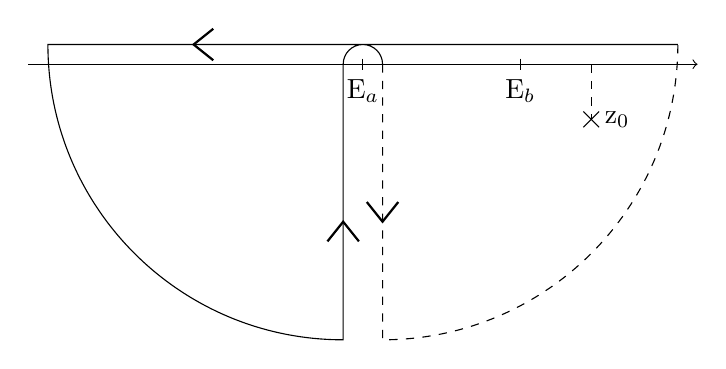
\begin{tikzpicture}
\draw [->] (-4.25,0) -- (4.25,0);
\draw (0,0.07) -- (0,-0.07) node [below]{E$_\mt{a}$};
\draw (2,0.07) -- (2,-0.07) node [below]{E$_\mt{b}$};
\draw [dashed] (2.9,0) --(2.9,-0.7);
\draw (2.95,-0.7)  node [right]{z$_0$};
\draw (2.8,-0.8) --(3,-0.6);
\draw (2.8,-0.6) --(3,-0.8);
\draw (4,0.25) -- (-4,0.25) arc (180:270:3.75) -- (-0.25,0)  arc (180:0:0.25);
\draw [dashed] (0.25,0) -- (0.25,-3.5) arc (270:360:3.75);
\draw [thick] (-1.9,0.45) -- (-2.15,0.25) -- (-1.9,0.05);
\draw [thick] (-0.45,-2.25) -- (-0.25,-2) -- (-0.05,-2.25);
\draw [thick] (0.45,-1.75) -- (0.25,-2) -- (0.05,-1.75);
\end{tikzpicture} \end{center}

Le long de ce contour $\mc{C}$, G$_\mt{b}$(z) est continu et on peut appliquer
le théorème des résidus. Or les seuls pôles de G$_\mt{b}$(z) ne peuvent, d'après
\S B 2°),se trouver que dans le deuxième feuillet de Riemann. Nous avons montré
l'existence d'un pôle z$_0$ situé sensiblement à la distance $\frac{\Gamma(\mt{E}_\mt{b})}{2}$ de l'axe réel.
Nous supposerons dans la suite que ce pôle est bien le seul. On peut alors compléter le contour  à l'aide d'un petit cercle orienté autour de z$_0$ et
écrire, à la limite où le rayon des quarts de cercle tend vers l'infini et
en explicitant l'intégrale du lacet :
% 245
\[
\tag{19} \frac{1}{2\mt{i}\pi}\int_\mt{C}\mt{G}_\mt{b}\mt{(z)}\mt{e}^{-\frac{\mt{izt}}{\hbar}}\mt{dz} =
\frac{1}{2\mt{i}\pi}\int_{\mt{E}_\mt{a}-\mt{i}\infty}^{\mt{E}_\mt{a}}\overline{\mt{G}_\mt{b}}\mt{(z)}\mt{e}^{-\frac{\mt{izt}}{\hbar}}\mt{dz} +
\frac{1}{2\mt{i}\pi}\int_{\mt{E}_\mt{a}}^{\mt{E}_\mt{a}-\mt{i}\infty}\mt{G}_\mt{b}\mt{(z)}\mt{e}^{-\frac{\mt{izt}}{\hbar}}\mt{dz}
\]
\[
+\mt{Résidu en z}_0 \left \{ \overline{\mt{G}_\mt{b}}\mt{(z)}\mt{e}^{-\frac{\mt{izt}}{\hbar}} \right \}
\]
%Intégrale le long du lacet
le contour d'intégration correspondant étant représenté par la figure ci-dessous
\begin{center} \begin{tikzpicture}
\draw [->] (-4.25,0) -- (4.25,0);
\draw (0,-0.07) -- (0,0.07) node [above right]{E$_\mt{a}$};
\draw (2,-0.07) -- (2,0.07) node [above]{E$_\mt{b}$};
\draw [dashed] (2.9,-0.7) circle(0.5);
\draw (2.95,-0.7)  node [below]{z$_0$};
\draw (2.8,-0.8) --(3,-0.6);
\draw (2.8,-0.6) --(3,-0.8);
\draw (-0.25,-3.5) -- (-0.25,0)  arc (180:0:0.25);
\draw [dashed] (0.25,0) -- (0.25,-3.5);
\draw [thick] (3.2,-0.5) -- (3.1,-0.25) -- (3.35,-0.20);
\draw [thick] (-0.45,-1.75) -- (-0.25,-2) -- (-0.05,-1.75);
\draw [thick] (0.45,-2.25) -- (0.25,-2) -- (0.05,-2.25);
\end{tikzpicture} \end{center}
\subsubsection{Calcul approché} %b) :

Nous justifierons plus bas que la contribution à L'expression (19) du lacet C' est en général négligeable. Nous n'en tiendrons pas
compte pour commencer et nous calculerons La contribution prépondérante du
résidu :

Soit $\overline{\mt{T}_\mt{b}}$(z) la détermination de $\mt{T}_\mt{b}$(z) dans le deuxième feuillet
de Riemann, Nous avons
% 246 —
\[
\overline{\mt{G}_\mt{b}}\mt{(z)}=\frac{1}{\mt{z}-\mt{E}_\mt{b}\overline{\mt{T}_\mt{b}}\mt{(z)}}
\]
et
\[
\tag{20}\mt{Résidu en z}_0 \left \{ \overline{\mt{G}_\mt{b}}\mt{(z)}\mt{e}^{-\frac{\mt{izt}}{\hbar}} \right \} =
\frac{1}{1-\left .\frac{\mt{d}\overline{\mt{T}_\mt{b}}\mt{(z)}}{\mt{dz}}\right |_{\mt{z}_0}}
\mt{e}^{-\frac{\mt{iz}_0\mt{t}}{\hbar}}
\]
L'expression (20) est rigoureuse. $\mt{T}_\mt{b}$(z) est peu différent de $\mt{T}_\mt{b}^\dagger$(E$_\mt{b}$).
C'est une quantité du deuxième ordre en $\mc{H}_\mt{I}$ dont les variations sont très
faibles et $\left .\frac{\mt{d}\overline{\mt{T}_\mt{b}}\mt{(z)}}{\mt{dz}}\right |_{\mt{z}_0}$ est absolument négligeable devant 1, si bien que
l'on peut écrire, si on néglige la contribution du lacet
\[
\tag{21}<\mt{b 0 }|\mt{ U(t) }|\mt{ b 0}> =
\frac{1}{2\mt{i}\pi}\int_\mt{C}\mt{G}_\mt{b}\mt{(z) e}^{-\frac{\mt{izt}}{\hbar}}
= \mt{e}^{-\frac{\mt{itz}_0}{\hbar}}
= \mt{e}^{-\mt{i}\frac{\mc{R}e(\mt{z}_0)\mt{t}}{\hbar}} \mt{e}^{-\mt{i}\frac{\mc{I}m(\mt{z}_0)\mt{t}}{\hbar}}
\]

Nous prévoyons ainsi, rigoureusement, et non plus par un calcul
au premier ordre du type "règle d'or de Fermi", que dans l'hypothèse de notre
modèle simple, l'état | b 0 > disparaît avec une constante de temps égale à
$\frac{\hbar}{2\mc{I}m(\mt{z}_0)}$
 et voit son énergie déplacée de la quantité $\mc{R}e(\mt{z}_0)-\mt{E}_\mt{b}$.
 
Nous pouvons maintenant, à une excellente approximation, remplacer
z$_0$ Par son expression (17) et écrire
\[
\tag{22}<\mt{b 0 }|\mt{ U(t) }|\mt{ b 0}> =
\mt{e}^{-\mt{it}\frac{\mt{E}_\mt{b}+\Delta(\mt{E}_\mt{b})}{\hbar}}
\mt{e}^{-\frac{\Gamma(\mt{E}_\mt{b})\mt{t}}{2\hbar}}
\]
% 247

$\Delta(\mt{E}_\mt{b})$ et $\Gamma(\mt{E}_\mt{b})$ étant donnés par les expressions (14-a) et (14-b) :
\[
\tag{23-a}\Delta(\mt{E}_\mt{b})=<\mc{P}\frac{1}
{\mt{E}_\mt{b}-\mt{E}_\mt{a}-\hbar\mt{ck}}\ ,
\mt{ k}^2\sum_\lambda\int\mt{d}\Omega\ |<\mt{ b 0 }|\ \mc{H}_\mt{I}\ |\mt{ a }\vec{\mt{k}}\ \lambda >|^2>
\]
\[
\tag{23-b}\Gamma(\mt{E}_\mt{b})=2\pi<\delta
(\mt{E}_\mt{b}-\mt{E}_\mt{a}-\hbar\mt{ck})\ ,
\mt{ k}^2\sum_\lambda\int\mt{d}\Omega\ |<\mt{ b 0 }|\ \mc{H}_\mt{I}\ |\mt{ a }\vec{\mt{k}}\ \lambda >|^2>
\]

Remarques : — la formule (23-b) n'est autre que celle que nous aurions
obtenue pour la durée de vie de l'état | b 0 > en appliquent la règle d'or
de Fermi. Le traitement que nous donnons ici nous permet cependant de prévoir le décroissance exponentielle rigoureuse à tous les ordres et l'existence d'un déplacement radiatif du niveau instable.

— l'intégrale (23-a) permettant de calculer $\Delta(\mt{E}_\mt{b})$ est divergente (terme croissant en k à l'infini). Cette divergence est due au fait
que nous traitons un système en interaction avec un champ (voir remarque de
la page 234 ) et disparaît si nous prenons pour la masse et la charge de
l'électron les masse et charge expérimentales.

\subsubsection{Ordre de grandeur de l'erreur faite en négligeant le lacet} %c)
Revenons maintenant à l'intégrale le long du lacet intervenant dans (19). Elle s'écrit :
\[
\tag{24}\mt{A}=\frac{1}{2\mt{i}\pi}
\int_{\mt{E}_\mt{a}}^{\mt{E}_\mt{a}-\mt{i}\infty}
\mt{e}^{-\frac{\mt{izt}}{\hbar}}\mt{dz}
\left [
\frac{1}{\mt{z}-\mt{E}_\mt{b}-\mt{T}_\mt{b}(\mt{z})}-
\frac{1}{\mt{z}-\mt{E}_\mt{b}-\overline{\mt{T}_\mt{b}}(\mt{z})}
\right ]
\]
\[
\ \ =\frac{1}{2\mt{i}\pi}\int_{\mt{E}_\mt{a}}^{\mt{E}_\mt{a}-\mt{i}\infty}
\mt{e}^{-\frac{\mt{izt}}{\hbar}}\ \frac{\overline{\mt{T}_\mt{b}}(\mt{z})-\mt{T}_\mt{b}(\mt{z})}
{(\mt{z}-\mt{E}_\mt{b}-\mt{T}_\mt{b}(\mt{z}))(\mt{z}-\mt{E}_\mt{b}-\overline{\mt{T}_\mt{b}}(\mt{z}))}\ \mt{dz}
\]
% 248 —
les quantités T$_\mt{b}$(z) et $\overline{\mt{T}_\mt{b}}$(z) sont des quantités petites du second ordre en
$\mc{H}_\mt{I}$, de l'ordre de $\Gamma_\mt{b}$ (nous posons  $\Gamma(\mt{E}_\mt{b})=\Gamma_\mt{b}$). D'autre part,
e$^{-\frac{\mt{izt}}{\hbar}}$
décroît très vite lorsque $|$ $\mc{I}m$ (z) $|$ augmente le long du lacet et on peut
majorer de façon très sévère $\mt{e}^{-\frac{\mt{izt}}{\hbar}}$ par 1. On a alors une majoration de A :
\[
\mt{A}<<\frac{1}{2\mt{i}\pi}\int_{\mt{E}_\mt{a}}^{\mt{E}_\mt{a}-\mt{i}\infty}
\frac{\Gamma_\mt{b}}{(\mt{z}-\mt{E}_\mt{b})^2}\ \mt{dz}=
\frac{1}{2\mt{i}\pi}\ \frac{\Gamma_\mt{b}}{\mt{E}_\mt{a}-\mt{E}_\mt{b}}
\]

Deux cas peuvent alors se présenter :

$\alpha$) Le temps t n'est pas trop long devant $\hbar/\Gamma_{b}$ : la contribution du résidu à
l'amplitude < b 0 $|$ U(t) $|$ b 0 > est de l'ordre de 1. L'erreur commise en négligeant
le lacet est alors négligeable dès que $\frac{\Gamma_\mt{b}}{\mt{E}_\mt{a}-\mt{E}_\mt{b}}$ << 1, c'est-à-dire dès
que la largeur naturelle du niveau b, $\Gamma_{b}$, est petite devant l'énergie de la
transition optique, ce qui est le cas la plupart du temps.

$\beta$) Le temps t est très grand : la contribution du résidu, en e$^\frac{\Gamma_{b}\mt{t}}{2}$, devient
très petite et la condition $\frac{\Gamma_\mt{b}}{\mt{E}_\mt{a}-\mt{E}_\mt{b}}$ << 1 n'est plus suffisante pour assurer que la correction apportée par le lacet à la loi de la décroissance exponentielle est négligeable.

De façon plus précise, lorsque t est très grand, seules les portions du contour d'intégration pour lesquelles $\mc{I}m$(z) est voisin de zéro interviennent de façon notable, c'est-à-dire d'après la figure de la page 245,
la partie du lacet voisine du point E$_\mt{a}$.

Alors que pour le pôle z$_0$, $|$ $\mc{I}m$ (z) $|$ est égal à $\Gamma_mt{b}$, on peut
trouver sur le lacet des points tels que $|$ $\mc{I}m$ (z) $|$ soit aussi petit que l'on
veut. Pour t très grand, le facteur e$^{-\frac{\mt{izt}}{\hbar}}$ atténue la contribution du pôle
beaucoup plus que celle du lacet. Il est donc intéressant dans ce cas d'étudier
le comportement de la contribution du lacet.

%249
La partie la plus importante de cette contribution correspondra
à y = $\mc{I}m$ (z) très petit. Les deux déterninations de T$_\mt{b}$(z) diffèrent alors pratiquement uniquement par leur partie imsginaire et on peut écrire
\begin{center}
T$_\mt{b}$(z) $-\ \overline{\mt{T}_\mt{b}}$(z) $\sim$ 2 $\mc{I}m$ ( E$_\mt{a}$ $+$ iy )
\end{center}

Or, d'après (12) :
\begin{center}
T$_\mt{b}$( E$_\mt{a}$ $+$ iy ) = $\int_0^\infty\frac{\mt{f(k)dk}}{\mt{iy} - \hbar\mt{ck}}$
\hspace{1cm} et \hspace{1cm}
2$\mc{I}m$ T$_\mt{b}$( E$_\mt{a}$ $+$ iy ) = -2y $\int_0^\infty\frac{\mt{f(k)dk}}{\mt{y}^2 + \hbar^2\mt{c}^2\mt{k}^2}$
\end{center}

Or d'après (11), f(k) varie comme k$^2$,
\begin{center}
$\int_0^\infty\frac{\mt{f(k)dk}}{\mt{y}^2 + \hbar^2\mt{c}^2\mt{k}^2}$
\hspace{1cm} se comporte comme \hspace{1cm}
$\int_0^\infty\frac{\mt{k}^2\mt{dk}}{\mt{y}^2 + \hbar^2\mt{c}^2\mt{k}^2}$
\end{center}
Soit, en faisant le changement de variable u = k/y,
comme y$\int_0^\infty\frac{\mt{du}}{1+ \hbar^2\mt{c}^2\mt{u}^2}$.
On en conclut donc que $\mc{I}m$ T$_\mt{b}$( E$_\mt{a}$ $+$ iy ) varie comme -y$^2$.

D'autre part, comme pour t très grand, la contribution la plus
importante à A dans (24) provient de z voisin de E$_\mt{a}$ on peut dans les dénominateurs remplacer z par E$_\mt{a}$. On a alors
\[
\mt{A}\simeq\frac{1}{2\mt{i}\pi}\ \frac{1}{(\mt{E}_\mt{a}-\mt{E}_\mt{b})^2}\int_0^\infty\mt{e}^{-\frac{\mt{yt}}{\hbar}}
\ 2\mc{I}m\ (\ \mt{T}_\mt{b}(\mt{E}_\mt{a}+\mt{iy})\ )\ \mt{dy},
\]
quantité qui varie donc comme $\int$e$^{-\frac{\mt{yt}}{\hbar}}$ y$^2$ dy.

% 250
En faisant enfin le changement de variable v $=$ ty, on a
$\int$e$^{-\frac{\mt{yt}}{\hbar}}$ y$^2$ dy $=\frac{1}{\mt{t}^3}\int$e$^{-\frac{\mt{v}}{\hbar}}$ v$^2$ dv
et on montre ainsi que, \ul{pour t très grand},
la contribution du lacet varie en $\frac{1}{\mt{t}^3}$.
{\footnotesize (On trouverait une contribution du lacet en 1/t$^{3/2}$ au lieu de 1/t$^{3}$ si on étudiait
la durée de vie d'un système sous l'effet de désintégration produisent des particules ayant
une masse \ul{différente de zéro}, et non des photons de \ul{masse nulle}, comme
c'est le cas dans l'émission spontanée.)}

Elle diminue donc beaucoup moins vite que la contribution du
résidu qui varie en e$^{-(\Gamma_\mt{b}\mt{t})/2\hbar}$.

On peut résumer les résultats précédents, en fonction du temps,
sur la figure ci-dessous. On a porté en ordonnée le module de la contribution
à $<$ b 0 $|$ U(t) $|$ b 0 $>$ du résidu (exponentielle en trait plein) et du lacet
(en trait pointillé).

\begin{center}
\begin{tikzpicture}
% Axes
\draw [thick, ->] (3,0) -- (3,4);
\draw [thick, ->] (3,0) -- (10,0) node [right]{t};
% Courbes
\def \A {200}
\draw [thick, domain=4:9, samples=100] plot (\x,{\A/exp(\x)});
\def \B {100}
\draw [thick, dashed, domain=4:9, samples=100] plot (\x,{\B/(\x^3)});
% Point
\draw [thick, dotted] (6.15,0.4) -- (6.15,0) node [below]{t$_0$};
\end{tikzpicture} \end{center}

% 251
On voit que cette dernière part, pour t $=$ 0, d'une quantité
de l'ordre de $\frac{\Gamma}{\mt{E}_\mt{a}-\mt{E}_\mt{b}}$
et décroit pour t très grand en 1/t$^3$. Pour un certain
temps t$_0$ \ul{très grand}, elle devient plus importante que celle de l'exponentielle.
Mais alors U$_\mt{b}$(t) est pratiquement nul et la désintégration est pour ainsi dire
terminée.

En d'autres termes, la loi de décroissance exponentielle de
l'état instable n'est pas \ul{théoriquement} vérifiée pour des temps très longs.
Elle l'est cependant tant que l'on est \ul{pratiquement} capable d'observer le processus de la désintégration.

\ul{Conclusion} : La contribution à l'évolution de l'état instable du pôle au point
z$_0$ est de loin la plus importante. Elle nous a permis de prévoir une durée de
vie et un déplacement radiatif de l'énergie de cet état. On néglige en général
la contribution du lacet introduit par la méthode des résidus, ce qui revient
à remplacer G$_\mt{b}$(z) par
\[
\frac{1}{\mt{z}-\mt{E}_\mt{b}-\mt{T}^+_\mt{b}(\mt{E}_\mt{b})}
\]
fonction analytique qui n'a plus de coupure mais qui présente un pôle au voisinage de z$_0$ au point
E$_\mt{b}+\Delta($E$_\mt{b})-i\frac{\Gamma(\mt{E}_\mt{b})}{2}$
\[
\tag{25}\frac{1}{\mt{z}-\mt{E}_\mt{b}-\mt{T}^+_\mt{b}(\mt{E}_\mt{b})}=
\frac{1}{\mt{z}-\mt{E}_\mt{b}-\Delta_\mt{b}+i(\Gamma_\mt{b}/2)}
\]
en posant $\Delta($E$_\mt{b})=\Delta_\mt{b}$ et $\Gamma($E$_\mt{b})=\Gamma_\mt{b}$.

\subsection{Produits de désintégration de l'état instable}% 4°)
Nous allons maintenant étudier les produits de la désintégration de
l'état $|$ b 0 $>$. Pour cela, il nous faut calculer l'amplitude de probabilité
$<$ a $\vec{\mt{k}}\ \lambda\ |$ U(t) $|$ b 0 $>$ pour que le système dans l'état $|$ b 0 $>$ à l'instant t $=$
0 se trouve dans l'état $|$ a $\vec{\mt{k}}\ \lambda>$ représentant l'atome dans l'état fondamental a
en présence d'un photon $\vec{\mt{k}}\,\lambda$, à l'instant t. Nous allons d'abord calculer la quantité
$<$ a $\vec{\mt{k}}\ \lambda\ |$ G(z) $|$ b 0 $>$.

% 252
\subsubsection{Etude de $<$ a $\vec{\mt{k}}\ \lambda\ |$ G(z) $|$ b 0 $>=$G$_{\mt{a}\vec{\mt{k}}\lambda,\mt{b}0}$}% a)
Nous partons de la relation G(z) $=$ G$_0$(z) $+$ G$_0$(z) $\mc{H}_\mt{I}$ G(z).
Etant donnée l'hypothèse simplificatrice, seuls les éléments de matrice
$<$ a $\vec{\mt{k}}\ \lambda\ |\ \mc{H}_\mt{I}\ |$ b 0 $>$ sont non nuls et on a, en adoptant l'expression (25)
pour G$_\mt{b}$(z)
\[
\tag{26}\mt{G}_{\mt{a}\vec{\mt{k}}\lambda,\mt{b}0}\mt{(z)}=
\frac{1}{\mt{z}-\mt{E}_\mt{a}-\hbar\mt{c}\mt{k}}
<\mt{a }\vec{\mt{k}}\ \lambda\ |\ \mc{H}_\mt{I}\ |\mt{ b } 0 >
\frac{1}{\mt{z}-\mt{E}_\mt{b}-\Delta_\mt{b}+i(\Gamma_\mt{b}/2)}
\]



\subsubsection{Etude de $<$ a $\vec{\mt{k}}\ \lambda\ |\ \mc{H}_\mt{I}\ |$ b 0 $>$}% b)
On calcule l'expression
\[
<\mt{a }\vec{\mt{k}}\ \lambda\ |\ \mt{U(t)}\ |\mt{ b } 0 >=\frac{1}{2\pi i}\int_\mt{c}
\mt{e}^{-\frac{i\mt{zt}}{\hbar}}\mt{G}_{\mt{a}\vec{\mt{k}}\lambda,\mt{b}0}\mt{(z) dz}
\]
par la méthode des résidus.

La quantité G$_{\mt{a}\vec{\mt{k}}\lambda,\mt{b}0}$(z) dz possède deux pôles, l'un au point E$_\mt{a}+\hbar$ck,
l'autre au point E$_\mt{b}+\Delta_\mt{b}-i(\Gamma_\mt{b}/2)$ et l'intégration par les résidus
donne :
\[
\tag{27}<\mt{a}\vec{\mt{k}}\lambda\,|\,\mt{U(t)}\,|\,\mt{b}0 >=
<\mt{a}\vec{\mt{k}}\lambda\,|\,\mc{H}_\mt{I}\,|\,\mt{b}0 >
\left[\frac{\mt{e}^{-i\frac{(\mt{E}_\mt{a}+\hbar\mt{ck)t}}{\hbar}}
-\mt{e}^{-i\frac{(\mt{E}_\mt{b}+\Delta(\mt{E}_\mt{b})\mt{)t}}{\hbar}}
\mt{e}^{-\frac{\Gamma_\mt{b}\mt{t}}{2\hbar}}}
{\hbar\mt{ck}-(\mt{E}_\mt{b}+\Delta_\mt{b}-\mt{E}_\mt{a})+i\frac{\Gamma_\mt{b}}{2}}\right]
\]

Pour des temps t grands devant $\hbar\Gamma_\mt{b}$ la première exponentielle
de (27), de module 1, est prépondérante et la probabilité de trouver un photon
$\vec{\mt{k}}\lambda$ émis est alors
\[
\tag{28}\mt{P}_{\vec{\mt{k}}\lambda}=\frac{|<\mt{a}\vec{\mt{k}}\lambda\,|\,\mc{H}_\mt{I}\,|\,\mt{b}\,0 >|^2}
{\big[\hbar\mt{ck}-(\mt{E}_\mt{b}+\Delta_\mt{b}-\mt{E}_\mt{a})\big]^2+\frac{\Gamma_\mt{b}^2}{4}}
\]

% 253

La formule (28) nous donne les propriétés de la raie d'émission spontanée à partir du niveau b :

- L'élément de matrice $<$ a $\vec{\mt{k}}\ \lambda\ |\ \mc{H}_\mt{I}\ |$ b 0 $>$ qui donne l'intensité de la raie, décrit la "force" de la transition
et contient toute l'information sur le diagramme d'émission (direction et polarisation des photons émis).

- Le dénominateur d'énergie indique que la raie est lorentzienne,
centrée pour une énergie du photon égale à la différence de l'énergie de l'état
excité corrigée par le déplacement radiatif $\Delta_\mt{b}$ et de l'état fondamental, de
largeur $\Gamma_\mt{b}$, inverse de la durée de vie de l'état excité. Tous ces résultats sont
en accord avec le principe de conservation de l'énergie et le relation d'incertitude.

\subsection{Etude de la diffusion résonnante}% 5°)



Nous allons maintenant rattacher l'étude de l'évolution de l'état
instable à celle de la diffusion résonnante des photons par un atome.
\subsubsection{Position du problème}% a)

Nous allons calculer la section efficace différentielle de diffusion d'un photon par un atome,
l'interaction électromagnétique entre l'atome
et les photons ne possédant, suivant l'hypothèse simplificatrice que nous avons
faite, que les éléments de matrice du type $<$ a $\vec{\mt{k}}\ \lambda\ |\ \mc{H}_\mt{I}\ |$ b 0 $>$ non nuls.
Dans ces conditions, la diffusion $\vec{\mt{k}}\lambda,\ \vec{\mt{k}}\,'\lambda'$, ne peut s'effectuer que par le
passage de l'atome de l'état a à l'état b par absorption du photon $\vec{\mt{k}}\lambda$ et la retombée de
l'état b à l'état a avec émission d'un photon $\vec{\mt{k}}\,'\lambda'$, suivant le schéma ci-dessous :
\begin{center} 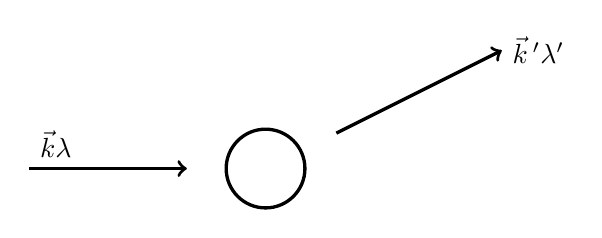
\begin{tikzpicture}
\draw [->, very thick] (-3,0) node [above right] {$\vec{\mt{k}}\lambda$} -- (-1,0);
\draw [->, very thick] (0.9,0.45) -- (3,1.5) node [right] {$\vec{\mt{k}}\,'\lambda'$};
\draw [very thick] (0, 0) circle (0.5);
\end{tikzpicture} \end{center}

% 254
Il est donc naturel de s'attendre à des phénomènes résonnants
lorsque l'énergie du photon incident sera de l'ordre de la différence d'énergie E$_\mt{b}-$E$_\mt{a}$.

Nous allons tout d'abord calculer l'élément de matrice de la
résolvante $<$ a $\vec{\mt{k}}\,'\ \lambda'\ |\mt{ G(z) }|$ a $\vec{\mt{k}}\ \lambda>\,=\,$
G$_{\mt{a}\vec{\mt{k}}\,'\lambda',\mt{a}\vec{\mt{k}}\lambda}$.
Nous pourrons alors évaluer l'amplitude de probabilité
$<$ a $\vec{\mt{k}}\,'\ \lambda'\ |\mt{ U(t) }|$ a $\vec{\mt{k}}\ \lambda>$ pour que l'atome
dans l'état fondamental a en présence d'un photon $\vec{\mt{k}}\lambda$ à l'instant $-$t/2 ait diffusé
à l'instant t/2 un photon $\vec{\mt{k}}\,'\lambda'$.

Nous avons vu (étude de la matrice S, chapitre 6)
que, pour t$\to\infty$, cette amplitude de probabilité n'admet pas de limite au
sens usuel, mais que si on passe en "représentation d'interaction"
$<$ a $\vec{\mt{k}}\,'\ \lambda'\ |\ \tilde{\mt{U}}\mt{(t) }|$ a $\vec{\mt{k}}\ \lambda>$
admet comme limite \ul{au sens des distributions} sur
les fonctions de $\vec{\mt{k}}$, l'élément de matrice S$_{\vec{\mt{k}}\,'\lambda',\,\vec{\mt{k}}\,\lambda}$.

Ayant calculé ainsi S$_{\vec{\mt{k}}\,'\lambda',\,\vec{\mt{k}}\,\lambda}$, nous en déduirons l'élément de
la matrice de réaction $\mc{R}_{\vec{\mt{k}}\,'\lambda',\,\vec{\mt{k}}\,\lambda}$ et la section efficace de diffusion.

\subsubsection{Calcul de G$_{\mt{a}\vec{\mt{k}}\,'\lambda',\,\mt{a}\vec{\mt{k}}\lambda}$}% b)
Partons des deux relations équivalentes
\[
\left\{ \begin{array}{rcl}
\mt{G} & = & \mt{G}_0+\mt{G}_0\,\mc{H}_\mt{I}\,\mt{G} \\
\mt{G} & = & \mt{G}_0+\mt{G}\,\mc{H}_\mt{I}\,\mt{G}_0 \end{array} \right.
\]
qui, combinées, donnent
\[
\tag{29}\mt{G}=\mt{G}_0+\mt{G}_0\,\mc{H}_\mt{I}\,\mt{G}_0+\mt{G}_0\,\mc{H}_\mt{I}\,\mt{G}\,\mc{H}_\mt{I}\,\mt{G}_0
\]
On obtient alors
\[
\mt{G}_{\mt{a}\vec{\mt{k}}\,'\lambda',\,\mt{a}\vec{\mt{k}}\lambda}=
\frac{\delta(\vec{\mt{k}}-\vec{\mt{k}}\,')\delta_{\lambda\lambda'}}{\mt{z}-\mt{E}_\mt{a}-\hbar\mt{ck}}+
\frac{<\mt{a}\vec{\mt{k}}\,'\lambda'\,|\,\mc{H}_\mt{I}\,|\,\mt{b}\,0 >\mt{G}_\mt{b}\mt{(z)}
<\mt{b}\,0\,|\,\mc{H}_\mt{I}\,|\,\mt{a}\vec{\mt{k}}\lambda>}
{(\mt{z}-\mt{E}_\mt{a}-\hbar\mt{ck'})(\mt{z}-\mt{E}_\mt{a}-\hbar\mt{ck})}
\]
% 255
Soit, en remplaçant G$_\mt{b}$(z) par son expression approchée (25) :
\[
\mt{G}_{\mt{a}\vec{\mt{k}}\,'\lambda',\,\mt{a}\vec{\mt{k}}\lambda}=
\frac{\delta(\vec{\mt{k}}-\vec{\mt{k}}\,')\delta_{\lambda\lambda'}}{\mt{z}-\mt{E}_\mt{a}-\hbar\mt{ck}}
\]
\[
\tag{30}+\frac{<\mt{a}\vec{\mt{k}}\,'\lambda'\,|\,\mc{H}_\mt{I}\,|\,\mt{b}\,0 >
<\mt{b}\,0\,|\,\mc{H}_\mt{I}\,|\,\mt{a}\vec{\mt{k}}\lambda>}
{(\mt{z}-\mt{E}_\mt{a}-\hbar\mt{ck'})(\mt{z}-\mt{E}_\mt{a}-\hbar\mt{ck})
(\mt{z}-\mt{E}_\mt{b}-\Delta_\mt{b}+i(\Gamma_\mt{b}/2))}
\]

\subsubsection{Calcul de $<$ a$\vec{\mt{k}}\,'\lambda'\,|$ U(t) $|$ a$\vec{\mt{k}}\lambda>$ et de la matrice S}% c)
Comme nous l'avons vu aux pages 149 et suivantes, il faut,
afin de calculer la matrice S, évaluer la limite au sens des distributions
pour t$\to\infty$ de $\tilde{\mt{U}}$ (t/2, $-$t/2), le signe $\tilde{ }$ dénotant la représentacion d'interaction.

Or, nous avons, d'après lu relation (82), chapitre 6 :
\[
\tag{31}\tilde{\mt{U}}(\mt{t}/2,-\mt{t}/2)=\mt{e}^{i\frac{\mt{H}_0}{2\hbar}\mt{t}}
\ \mt{U}(\mt{t}/2,-\mt{t}/2)\ \mt{e}^{i\frac{\mt{H}_0}{2\hbar}\mt{t}}
\]

Nous devons done commencer par calculer les éléments de matrice de U(t/2, $-$t/2)
Nous savons d'autre part que U(t/2, $-$t/2)$=$e$^{-i\frac{H}{\hbar}(\mt{t}/2+\mt{t}/2)}=$
e$^{-i\frac{H}{\hbar}\mt{t}}=$U(t,0).
Nous sommes donc ramenés au calcul de l'élément de matrice
$<$ a$\vec{\mt{k}}\,'\lambda'\,|$ U(t) $|$ a$\vec{\mt{k}}\lambda>$
que nous évaluerons par les résidus à partir de la relation
\[
<\mt{a}\vec{\mt{k}}\,'\lambda'\,|\mt{ U(t) }|\,\mt{a}\vec{\mt{k}}\lambda>=\frac{1}{2i\pi}\int_\mt{c}\mt{e}
^{-i\frac{\mt{zt}}{\hbar}}\mt{G}_{\mt{a}\vec{\mt{k}}\,'\lambda',\,\mt{a}\vec{\mt{k}}\lambda}\mt{(z) dz}
\]
La contribution du premier terme du second. membre de (30) donne immédiatement
\[
\mt{e}^{-i\frac{(\mt{E}_\mt{a}+\hbar\mt{ck)t}}{\hbar}}\delta(\vec{\mt{k}}-\vec{\mt{k}}\,')\delta_{\lambda\lambda'}
\]

Comme nous allons être amenés à prendre la limite pour t$\to\infty$
de l'expression obtenue, nous pouvons dans la contribution du second terme de
(30) négliger le résidu du pôle z$_0=$E$_\mt{b}+\Delta_\mt{b}-i\frac{\Gamma_\mt{b}}{2}$
dont le module décroît en e$^{-\frac{\Gamma_\mt{b}\mt{t}}{2\hbar}}$.
% 256
On ne tiendra compte finalement que des résidus des pôles z $=$ E$_\mt{a}+\hbar$ck et z $=$ E$_\mt{a}+\hbar$ck'.

On obtient alors
\[
<\mt{a}\vec{\mt{k}}\,'\lambda'\,|\mt{ U(t) }|\,\mt{a}\vec{\mt{k}}\lambda>=
\delta(\vec{\mt{k}}-\vec{\mt{k}}\,')\delta_{\lambda\lambda'}
\,\mt{e}^{-i\frac{(\mt{E}_\mt{a}+\hbar\mt{ck)t}}{\hbar}}\ +
\]
\[
<\mt{a}\vec{\mt{k}}\,'\lambda'\,|\,\mc{H}_\mt{I}\,|\,\mt{b}\,0 >
<\mt{b}\,0\,|\,\mc{H}_\mt{I}\,|\,\mt{a}\vec{\mt{k}}\lambda>\left[
\frac{\mt{e}^{-i\frac{(\mt{E}_\mt{a}+\hbar\mt{ck)t}}{\hbar}}}{\hbar\mt{c(k}-\mt{k')}}
\ \frac{1}{\hbar\mt{ck}+\mt{E}_\mt{a}-\mt{E}_\mt{b}-\Delta_\mt{b}+i(\Gamma_\mt{b}/2)}
\right .
\]
\[
\tag{32-a}-\ \left.
\frac{\mt{e}^{-i\frac{(\mt{E}_\mt{a}+\hbar\mt{ck')t}}{\hbar}}}{\hbar\mt{c(k}-\mt{k')}}
\ \frac{1}{\hbar\mt{ck'}+\mt{E}_\mt{a}-\mt{E}_\mt{b}-\Delta_\mt{b}+i(\Gamma_\mt{b}/2)}
\right]
\]

La relation (32-a) s'écrit, en remarquant que l'on peut, dans le premier
terme, en raison de la distribution $\delta(\vec{\mt{k}}-\vec{\mt{k}}\,')$, remplacer
e$^{-i\frac{(\mt{E}_\mt{a}+\hbar\mt{ck)t}}{\hbar}}$ par
e$^{-\frac{i}{\hbar}\left[\mt{E}_\mt{a}+\hbar\mt{c}\frac{(\mt{k}+\mt{k')t}}{2}\right]}$ et que
\[
\left\{ \begin{array}{rcl}
\mt{E}_\mt{a}+\hbar\mt{ck} & = & \mt{E}_\mt{a}+\hbar\mt{c}\frac{(\mt{k}+\mt{k')}}{2}
+\hbar\mt{c}\frac{(\mt{k}-\mt{k')}}{2} \\
\mt{E}_\mt{a}+\hbar\mt{ck'} & = & \mt{E}_\mt{a}+\hbar\mt{c}\frac{(\mt{k}+\mt{k')}}{2}
+\hbar\mt{c}\frac{(\mt{k'}-\mt{k)}}{2} \end{array} \right.
\]
% 257
\[
<\mt{a}\vec{\mt{k}}\,'\lambda'\,|\mt{ U(t) }|\,\mt{a}\vec{\mt{k}}\lambda>=
<\mt{a}\vec{\mt{k}}\,'\lambda'\,|\mt{ U}(\frac{\mt{t}}{2},\ -\frac{\mt{t}}{2}) |\,\mt{a}\vec{\mt{k}}\lambda>
\]
\[
=\mt{exp}-\frac{i}{\hbar}\left[\mt{E}_\mt{a}+\hbar\mt{c}\frac{\mt{(k}+\mt{k}')}{2}\mt{t}\right]
\ \delta(\vec{\mt{k}}-\vec{\mt{k}}\,')\ \delta_{\lambda\lambda'}
\]
\[
+\mt{ exp}-\frac{i}{\hbar}\left[\mt{E}_\mt{a}+\hbar\mt{c}\frac{\mt{(k}+\mt{k}')}{2}\mt{t}\right]
<\mt{a}\vec{\mt{k}}\,'\lambda'\,|\,\mc{H}_\mt{I}\,|\,\mt{b }0>
<\mt{b }0\,|\,\mc{H}_\mt{I}\,|\,\mt{a}\vec{\mt{k}}\lambda>\times
\]
\[
\left[
\frac{\mt{e}^{-i\hbar\mt{c}\frac{\mt{(k}-\mt{k}')}{2\hbar}\mt{t}}}{\hbar\mt{c(k}-\mt{k')}}
\ \frac{1}{\hbar\mt{ck}+\mt{E}_\mt{a}-\mt{E}_\mt{b}-\Delta_\mt{b}+i(\Gamma_\mt{b}/2)}
\right .
\]
\[
\tag{32-b}-\ \left.
\frac{\mt{e}^{-i\hbar\mt{c}\frac{\mt{(k}-\mt{k}')}{2\hbar}\mt{t}}}{\hbar\mt{c(k}-\mt{k')}}
\ \frac{1}{\hbar\mt{ck'}+\mt{E}_\mt{a}-\mt{E}_\mt{b}-\Delta_\mt{b}+i(\Gamma_\mt{b}/2)}
\right]
\]

Passons maintenant en représentation d'interaction. (31) s'écrit :
\[
<\mt{a}\vec{\mt{k}}\,'\lambda'\,|\tilde{\mt{U}}(\frac{\mt{t}}{2},\ -\frac{\mt{t}}{2})|\,\mt{a}\vec{\mt{k}}\lambda>=
\mt{e}^{-\frac{i}{2\hbar}\left[\mt{E}_\mt{a}+\hbar\mt{ck}'\right]\mt{t}}
<\mt{a}\vec{\mt{k}}\,'\lambda'\,|\mt{ U}(\mt{t) }|\,\mt{a}\vec{\mt{k}}\lambda>
\mt{e}^{-\frac{i}{2\hbar}\big[\mt{E}_\mt{a}+\hbar\mt{ck}\big]\mt{t}}
\]
\[
=\mt{exp }\frac{i}{\hbar}\left[\mt{E}_\mt{a}+\hbar\mt{c}\frac{\mt{(k}+\mt{k}')}{2}\right]\mt{t}
<\mt{a}\vec{\mt{k}}\,'\lambda'\,|\mt{ U}(\mt{t) }|\,\mt{a}\vec{\mt{k}}\lambda>
\]

Le passage en représentation d'interaction revient donc à supprimer Le terme
de phase exp $-\frac{i}{\hbar}\left[\mt{E}_\mt{a}+\hbar\mt{c}\frac{\mt{(k}+\mt{k}')}{2}\right]\mt{t}$ 
qui est en facteur dans l'expression (32-b)
et on obtient finalement :
\[
<\mt{a}\vec{\mt{k}}\,'\lambda'\,|\tilde{\mt{U}}(\frac{\mt{t}}{2},\ -\frac{\mt{t}}{2})|\,\mt{a}\vec{\mt{k}}\lambda>\ =
\ \delta(\vec{\mt{k}}-\vec{\mt{k}}\,')\ \delta_{\lambda\lambda'}\ +
\]
\[
<\mt{a}\vec{\mt{k}}\,'\lambda'\,|\,\mc{H}_\mt{I}\,|\,\mt{b}\,0 >
<\mt{b}\,0\,|\,\mc{H}_\mt{I}\,|\,\mt{a}\vec{\mt{k}}\lambda>\left[
\frac{\mt{e}^{-i\,\hbar\mt{c}\,\frac{\mt{c(k}-\mt{k')}}{2\hbar}\mt{t}}}{\hbar\mt{c(k}-\mt{k')}}
\ \frac{1}{\hbar\mt{ck}+\mt{E}_\mt{a}-\mt{E}_\mt{b}-\Delta_\mt{b}+i(\Gamma_\mt{b}/2)}
\right .
\]
\[
\tag{33}-\ \left.
\frac{\mt{e}^{-i\,\hbar\mt{c}\,\frac{\mt{c(k}-\mt{k')}}{2\hbar}\mt{t}}}{\hbar\mt{c(k}-\mt{k')}}
\ \frac{1}{\hbar\mt{ck'}+\mt{E}_\mt{a}-\mt{E}_\mt{b}-\Delta_\mt{b}+i(\Gamma_\mt{b}/2)}
\right]
\]

% 258
Séparons dans le crochet du second membre de (33) les parties
réelles et imaginaires des exponentielles. Le terme associé aux parties réelles,
A, s'écrit :
\[
\mt{A}=\frac{\mt{cos c }\frac{\mt{(k}-\mt{k')}}{2}\mt{t}}{\hbar\mt{c (k}-\mt{k')}}
\left[\ \frac{1}{\hbar\mt{ck}+\mt{E}_\mt{a}-\mt{E}_\mt{b}-\Delta_\mt{b}+i(\Gamma_\mt{b}/2)}\right.
\]
\[
\left.-\ \frac{1}{\hbar\mt{ck'}+\mt{E}_\mt{a}-\mt{E}_\mt{b}-\Delta_\mt{b}+i(\Gamma_\mt{b}/2)}\right]
\]
\[
=-\,\mt{cos c }\frac{\mt{(k}-\mt{k')}}{2}\mt{ t }\times
\]
\[
\frac{1}{(\hbar\mt{ck}+\mt{E}_\mt{a}-\mt{E}_\mt{b}-\Delta_\mt{b}+i(\Gamma_\mt{b}/2))
(\hbar\mt{ck'}+\mt{E}_\mt{a}-\mt{E}_\mt{b}-\Delta_\mt{b}+i(\Gamma_\mt{b}/2))}
\]


C'est une fonction de k et k' qui reste bornée quel que soit t.
Lorsque t augmente indéfiniment, sa période, $4\pi/$ct, tend vers zéro et la fonction oscille de plus en plus vite. L'intégrale de son produit par une autre
fonction sommable tend donc vers zéro lorsque t$\to\infty$ et \ul{A tend vers zéro au
sens des distributions sur les fonctions de k et k'} :
\[
\tag{34-a}\lim_{\mt{t}\to\infty}\mt{A}=0
\]
Le terme associé aux parties imaginaires, B, s'écrit :
\[
\tag{34-b}\mt{B}=-\,\mt{cos c }\frac{\mt{(k}-\mt{k')}}{2}\mt{ t }\times
\]
\[
\frac{1}{(\hbar\mt{ck}+\mt{E}_\mt{a}-\mt{E}_\mt{b}-\Delta_\mt{b}+i(\Gamma_\mt{b}/2))
(\hbar\mt{ck'}+\mt{E}_\mt{a}-\mt{E}_\mt{b}-\Delta_\mt{b}+i(\Gamma_\mt{b}/2))}
\]

Or, nous savons a'après p. 152 et 153) que la limite au sens des distributions

sin ce (k-k') 
lorsque t + « de tr) est égale à 

Le présence de la distribution 6 permettant de poser k = k' dans

(3k-b), on a finalement

% 259

On a donc, d'après (33), (3h-a) et (3k-ce) :



(35) 

(35) nous donne pour l'élément de la matrice  une relation strictement
équivalente à la relation (28), page 107 :
On en déduit immédiatement l'élément de matrice de réaction :


Remarque : la relation (36) pouvait s'établir beaucoup plus rapidement en par
tent de la relation qui définit la matrice de réaction ‘:

et en prenant pour > la forme explicite :

On obtient alors

Or  est autre que G. Nous avons donc
(38)
Si on prend pour * la forme approchée (2%, (38) redonne (36).

(39)
% 260 —

\subsubsection{} Calcul de la section efficace de diffusion%d)

 permet de calculer la probabilité de transition

par mité de temps de l'état KA à l'état K'A' (cf formules (68) pe 136 ou

La probabilité de transition par unité de temps et d'angle

solide W () s'obtient en sommant sur le module du vecteur d'onde k

(cf formule (69) p. 137)

Le flux du photon incident est et la section efficace

de diffusion s'écrit, compte tenu de (36) et (40)

Nous voyons ainsi que les éléments de matrice S (formule 35),
BR (formule 36) et 1a section efficace différentielle de diffusion (formule 41)

subissent une résonence lorsque l'énergie du photon incident est égale à la
différence des énergies de l'état excité corripée par le déplacement rediatif
A, et de l'état fondamental. La courbe. de résonance de la section efficace est

lorentzienne, de larseur l, érale à la larseur naturelle de l'état excité.
% 261

Nous avons vu également que l'énergie du photon diffusé est
égale à celle du photon incident (à cause de la fonction 6) ce qui correspond au principe de conservation de l'énergiee

Le diagramme d'impulsion et de polarisation du rayonnement

diffusé est fourni par le produit des éléments de matrice d'interaction

\subsection{} Préparation de l'état instable :%6°)
Nous avons, grêüce au calcul de G  commencé
par étudier l'émission spontanée à partir d'un niveau instable b, responsabie

de la durée de vie de cet état. Puis, grâce au calcul de G Nous avons

étudié le diffusion des photons par un atome à deux niveaux  et Do Afin que
notre étude soit complète, il nous faut maintenant étudier l'absorption d'un
photon par l'atome passant de l'état fondemental à J'état excité b. Cette
étude fait intervenir le dernier élément de matrice non calculé de ‘la résolvante, G, a° Elle est importante car elle nous décrit la préparation de
l'état excité et nous montre dans quelles conditions il est possible de 5éparer la préparation de l'état instable de sa désintégration et done de donner
un sens à le notion de durée de vie de l'état excité

Nous envoyons sur l'atome un ‘paquet d'onde de photons" de
polarisation À et d'impulsion centrée autour d'une valeur k avec une disper
sion 4k que l'on peut noter

f(k) est une fonction centrée en k, de largeur Ak qui représente le profil de
le raie excitatrice. Nous envisageons ici uniquement une dispersion en module
du vecteur d'onde, et non en direction.

A l'instant t = O, l'atome est dans l'état fondamental a en

présence du paquet d'onde
% 262 —

L'amplitude de probabilité pour qu'il soit à l'instant t dans

l'état | b O > est

Or nous avons

et  calcule comme  (cf p.252 , formule 26)

- Faisons l'hypothèse que l'élément de matrice 

varie peu le long du profil de la raie excitatrice et calculons

 Compte tenu de (L2), (43) et (kh) à l'aide de la méthode
des résidus. Il vient finalement

Afin de rendre l'expression (k5) plus maniable, nous allons dé
finir la transformée de Fourier de la fonction f (k) par la relation

car nous pouvons toujours supposer que f(k) est identiquement nulle pour k < 0.

(47)

(48)

(49)

(50)

% 263
On a de même :

 étant la fonction échelon : 

comme il est facile de s'en rendre compte en intégrant per lu méthode des
résidus. On peut alors considérer les deux intégrales intervenant dans (45)
comme des transformées de Fourier prises aux instants O et t d'un produit de
fonction de k et en se servant du fait que la transformée de Fourier d'un
produit est égale au produit de convolution des transformées de Fourier, on

montre aisément la relation :

qui pour t = O s'écrit :

A l'aide de (48) et (49), (h5) s'écrit ;

ou encore

(r) étant donné par la relation (L6),

% 264

Lorsque t = 0, les deux bornes de l'intégrale de (50) sont
égeles à zéro : on retrouve le fait évident que l'amplitude de probabilité
d'excitation est nulle à l'instant t = O.

Afin d'étudier comment cette amplitude de probabilité varie
avec le temps, nous allons distinguer deux cas fondamentalement différents :
\subsection{} Excitation "Narrow-line" :%a)
La largeur de la raie excitatrice Ak est très
petite devant TL,  on excite à l'aide d'une raie très fine, On peut alors
considérer que f(k) est la distribution 6 (k-k)s On a alors

ce qui reporté dans (50) nous donne pour amplitude de probabilité :

(51)

Après un régime transitoire durant un temps de l'ordre de AT,

la deuxième exponentielle du crochet de (51) devient négligeable devant la
première dont le module est égal à 1 et on peut alors écrire la probabilité

P, de trouver l'atome dans l'état excité b :

Le varietion de Pen fonction du temps est représentée par la figure ci-dessous :

% 265
Après un régime transitoire durant un temps de l'ordre de
HT,» la probabilité de trouver l'atome dans l'état excité prend une valeur
constante d'autant plus grande que la fréquence du photon est plus proche de

 On ne peut pas parler de durée de vie



la fréquence atomique
de l'état excité.
Ceci se comprend très aisément : la raie d'excitation étant
très fine, le temps de passage du photon devant l'atome (donné par 1a largeur
de la transformée de Fourier  (tr) ) est très grand : en termes classiques,
l'atome voit passer une onde plane qui, après un régime transitoire durant le
temps UT, met le dipôle électrique atomique en vibration forcée. La probabilité de trouver l'atome dans l'état excité est alors une constante qui devient
très importante lorsque l'excitation du dipôle est résonnante, c'est-ü-dire
lorsque 1a fréquence d'excitation est égale à la fréquence propre atomique.
\subsection{} Excitation "Broad-line" :%b)
Supposons maintenant, au contraire, que la largeur de la raie
excitatrice Ak est très grande devant la largeur naturelle :

Corrélativement, la transformée de Fourier âu profil de la raie
d'excitation, (rt), aura une largeur très faible, T, de l'ordre de  << E..

T représente physiquement le temps de passage du train d'onde sur l'atome.
On peut toujours écrire  (tr) en introduisant la fréquence
moyenne k de la raie d'excitation

où g a le largeur T de.

(50) s'écrit alors

(53)

% 266
Dès que t devient égal à un certain instant T tel que
 est sensiblement nul et l'intégrale de l'expression (53)



Th 1
peut être remplacée par l'intégrale définie

, laquelle, puisque T, << Te

est sensiblement égale à
dr. Cette intégrale est indépendante
du temps et le seul facteur dépendant du temps dans reste

alors le facteur e dont le module décroît en
D'autre part l'intégrant de l'intégrale définie I est le

produit de g (tr), de largeur T par un facteur de phase de fréquence
 « 11 sera donc une fonction de k maximum pour 
et qui s'annulera lorsque le nombre d'oscillations du facteur oscillant sur la
largeur T de g (tr) sera très grand, c'est-à-dire dès que

 de largeur

Afin de résumer les résultats précédents, les variations de

sera donc une fonction de k centrée en

sont schématisées sur la figure ci-dessous :

% 267
On voit que pendant un temps de l'ordre de T à partir de t =
(temps de passage du train d'onde sur l'atome) la probnbilité augmente, ce
qui correspond à l'excitation de l'atome par le train d'onde, Puis, la probabilité passe par un maximum et décroît exponentiellement avec une constante de
temps H/T,s ce qui correspond à la phase de désintégration de l'état excité
sous l'effet de l'émission spontanée.

Le maximum de la probabilité d'excitation est lui-même une fonction de la fréquence moyenne k du train d'onde excitateur, maximale lorsque la

largeur sensible

fréquence k est égale à la fréquence atomique
ment égale à Ak, largeur de la raie excitatrices

Tous ces résultats sont en accord avec le principe de conserva
tion de l'énergie et la relation d'incertitude.
En résumé, l'excitation “broad-line" est une excitation ‘en

pulse" qui permet de séparer les pheses de préparation et de désintégration de
l'état excité. Ce n'est qu'avec une telle préparation qu'il est possible de onner un sens à la notion de durée de vie de l'état excité.

Remarque : Il est possible de calculer entièrement le modèle d'excitation "broad-line"
en prenant pour profil de la raie excitatrice une raie de Lorentz centrée en k
de largeur 4k. On a alors

et on peut calculer rigoureusement l'expression (53) :

On trouve, en négligeant Th devant Ak dans le dénomineteur résonnant :

% 268

Le dénominateur d'énergie nous montre que le maximum de probabilité d'exciteti ARS nt un profil de Lorentz centré en k = 
largeur ,

Le premier terme du crochet est un terme de "préparation" qui
disparaît après un temps de l'ordre de T =  Le second est le terme de
désintégration de l'état excité.

Tous ces résultats illustrent les considérations générales faites à propos de l'excitation "broad-line".

\section{} Etude du cas général.%C.
\subsection{} Introduction :%1°)

Dans le traitement que nous avons présenté au  B, l'hypothèse
que seuls les éléments de matrice < a | | bO > sont différents de zéro
nous a permis de nous limiter au sous-espace É, sous-tendu par | b O > et
| a > et le calcul des éléments de matrice de G(z) revenait à inverser dans

ce sous=espace la matrice z = H :

% 269
En fait , possède d'autres éléments de matrice que
.
D'une part, | bO > peut être 1ié à des états |  >, (ce étant,
un état atomique autre que a); les processus correspondants seront importants
si l'énergie de l'état c se trouve comprise entre celles des états b et a, et
il y aura possibilité d'émission spontanée de b vers Ce

D'autre part, l'état | ak > pourra être lié à des états à deux
photons du type |  >, ce couplage étant le cause d'un déplacement
d'énergie de l'état fondamental par émission et réabsorption virtuelles de
photons

Pour tenir compte de tous ces couplages, nous alïons utiliser
une méthode analogue à. celle qui nous a permis de généreliser la formule de
Rabi dans le chapitre sur les états discrets (cf pe 210 Je

Nous allons considérer la restriction G de G au sous-espace é,
sous-tendu par | bO > et | ak > et montrer que ê est l'inverse d'un opérateur
de ce sous-espace,  L'opérateur  contient les effects du couplage
des vecteurs d'état de é, avec tous les autres vecteurs. Ce couplage a pour
effet d' "habiller" les états | bO > et | aka >, et donc modifie leurs énergies.
Il modifie également le couplage entre les états de ER en "habiliant" 
ments de matrice d'interaction.

Nous commençons par définir, de façon analogue au chapitre sur
les états discrets (p. 210 ), des opérateurs F et R relatifs au sous-espace 
ce qui nous permet de donner une forme condensée de cz) (c-),

Puis nous étudions à l'aide d'une représentation diagrammatique
la restriction à de R à l'espace , (c-3),

Enfin, nous reprenons point par point, en indiquent les modifications apportées, l'étude que nous avons faite au  B de l'évolution de l'État instable ( C-k), de la raie d'émission spontanée vers l'état fondamental ( C-5)

et de la diffusion résonnante ( C-6).

% 270

\subsection{} Définition des opérateurs F et R. Calcul de G(z) :%2°)
\subsubsection{} Définitions Rappelons d'abord la définition des projecteurs%a)

Nous procédons ensuite exactement comme à la page 210 :

Nous posons
,
Nous définissons ensuite F(z) par la relation

commutant avec P, on peut écrire
(55-b)
De (55-b), on déduit

(56)

Nous définissons alors R(z) P, per la relation

et nous appelons R(z) la projection de R(z) dans le sous-espace 6. :

\subsubsection{} Calcul de F(z) et R(z)%b)
Nous calculons F(z) P, comme à la page 212 et nous en

déduisons d'après la relation (kh) de cette page :

(60)

(61)

(62)

(63)

% 271

(53) se développe en série de puissance de .

On a de même (relation 45, p. 212) :

où l'on peut déduire le développement de Yigner-Brillouin de R(z) :

\subsection{} Caleul de G(z)%c)
On montre comme à la page 211, relation :

(63) signifie que dans le sous-espace  opérateur G(z) est l'inverse de

Dans le modèle simple du  B, G(z) était l'inverse de
Nous sommes donc ramenés à un problème analogue à celui du  B, circonscrit
au sous-espace à condition de remplacer 8. par R(z)
\subsection{} Étude de H(z) :%3)
\subsubsection{} Représentation diagremmatique des éléments de matrice
de R(z)%a)
Le développement de R(z) en série des puissances de ,
est représenté par la formule (62) Nous voyons que pour calculer à un ordre n

déterminé l'élément de matrice de R(z) entre deux états de be il faut passer
par n-1 états intermédiaires situés en dehors de É, et diviser par les dénominateurs d'énergie correspondants.

Nous pouvons représenter chaque terme du développement d'un élément
de matrice de K(z) par des diagrammes qui permettront de "visualiser" le processus

physique correspondant à ce terme.

%272
Donnons-en quelques exemples :

nu
Soit à représenter l'élément de matrice < a(z)bO >

Le terme du ler ordre est, d'après (62)

KA
: ésentons nn
< aka [dB [bo > que nous représentons par le diagramme

Le terme du 3e ordre comprend par exemple l'expression :

-(Ce n'est pas là la seule contribution au terme du 3e ordre.
On doit, par exemple, également envisager les expressions dans lesquelles
interviennent des états intermédiaires à deux photons.)
Cependant, nous représentons l'expression (6k-a) par le diagramme

Ces deux exemples nous montrent clairement comment les diagrammes sont construits et nous permettent de préciser les règles suivantes :
- Chaque diagramme correspond à une expression intervenant dens le terme à un
ordre déterminé du développement d'un élément de matrice de É(z) suivant

l'expression (62).

Le diagramme se lit dans le même sens que l'élément de matrice correspondant,

Les états atomiques sont représentés par des traits horizontaux et les photons
par des "tortillons".
Les extrémités du diagramme sont les mêmes que celles de l'élément de matrice.

Chaque élément de matrice de e. correspondant à une interaction est repré
senté par un ronde

- Les états intermédiaires sont les mêmes que ceux de l'expression représentée,

Pour obtenir l'expression correspondante à chaque diagremme, il faut diviser

c'est-à-dire qu'ils doivent être tous extérieurs à

le produit des éléments de matrice par autant de dénominateurs d'énergie qu'il
y a d'états intermédiaires dans le diagramme (chaque dénominateur d'énergie
s'écrivant z = E, E étant l'énergie de l'état intermédieire envisagé) et
gommer sur tous les étuts intermédiaires possibles (c'est-ä-dire sur tous les
états intermédiaires extérieurs à 8 et représentés sur le diagramme),

Pour obtenir les éléments de matrice de R(z ), i1 faut sommer
tous les diagrammes possibles à un ordre déterminé et à tous les ordres:

Cette représentation diagranmatique permet d'écrire ce façon
condensée les éléments de matrice de Az) et surtout d'expliciter les proces=
sus physiques correspondant à un élément de matrice et à un ordre déterminés.
Ainsi, pour le diagramme (6h-b), l'atome dans 1'état b émet un photon
et passe dans l'état ca; puis il réabsorbe ce photon et passe dans l'état
db; enfin il émet un photon kÀA en passant dans l'état a.

L'hypothèse simplificatrice du  B revenait à remplacer X(z )
par son expression au prenier ordre, P 4 Poe

Nous allons ici nous attacher à étudier la correction au 2e
ordre aux résultats simples obtenus. Ceci nous permettra de dégager des résultats physiques simples et intéressants. Le calcul aux orûres supérieurs, quoique
plus long, ne présente pas de difficultés et s'effectuerait de la même manière o

Nous allons commencer par expliciter le développement de R(z) au

2e ordre inclus en ..
%274

\subsubsection{} Développement de R(2) au 2e ordre inclus en ,%b)
Hz) présente Fe types différents d'éléments de

matrice : 

Au deuxième ordre inclus : Ka
(z) est représenté per
b est représenté par (1)

quelconques

I1 est facile de voir qu'au second ordre inclus, seuls les six

diagrammes précédents sont possibles. Nous pouvons faire plusieurs remarques :
% 275 =

Nu
a) Seuls les diagrammes représentant RE D et Bi etx sont au premier ordre :

c'étaient ‘eux qui intervenaient dans le traitement du  B.:

8) Le diagramme (k) n'est possible que si les photons extrêmes sont identiques,
Le photon. KA joue alors le rôle de "spectateur" et n'intervient pes dons les
processus d'interaction. Les diagremmes (5) et (6) sunt possibles ausle que
soient les photons KA et k'A'.

y) Les photons de même K et À, en taut que bosons, sont des particules indis…
cernables. Or il n'a pas été tenu compte de l'indiscernabilité pour éteblir

les diagrammes précédents. IL est évident notamment que les diagrammes

correspondant au même processus physique sont équivalents et ne doivent être
comptés qu'une fois. Nous verrons au c) comment résoudre cette difficulté.
\subsection{} Séparation de R(z) en deux parties%c)

- Définition de R'(z) et R'"(z)

Posons par définition

Nous avons ainsi séparé R(z) = R(z) + R(z) en deux parties,

dont l'une, R(z), est diagonale.

(66)

(67)
% 276

Etude de R(z)

Nous allons montrer que les éléments de matrice

sont reliés très simplement à des quantités intervenant dans le calcul de la
self énergie de l'état fondamental.

Etudions pour cela la modification apportée par ie couplage
électromagnétique à l'état fondamental | a0 > et à son énergie.

Nous sommes amenés, comme nous l'avons fait dans le chapitre sur
les états discrets, à définir les projecteurs P, = | 20 > < a0 | et Q=l1-P,
sur l'état normé | a0 > et dans l'espace complémentaire, puis à définir

1 "Opérateur Shift" À, dont le développement de Wigner Brillouin est

. Pitoce
ce qui, à l'ordre le plus bas, donne

On montre iverente comme nous l'avons fait au  B que

et que  est une fonction analytique dans tout le plan complexe privé

d'une coupure partant de. étant l'énergie atomique la plus basse
au-dessus de l'état fondamental, E, étant inférieur à est analy



tique au point E a t par (68), on voit tout de suite que .

Il est même réget tif, car on voit sur l'expression (67) que tous Les dénominateurs d'énergies  sont négatifs.

% 277
(69)

(70)

(71)

On peut alors calculer l'élément de matrice de la résolvante

Les pôles de G (2) vérifient l'équation implicite

Il existe notamment une valeur propre ë, voisine de E, qui vérifie l'équation

dans laquelle on peut, à une bonne approximation, remplacer

par
On obtient alors

ce qui montre que sous l'effet de l'interaction électromagnétique, l'état
fondamental se trouve "habillé" par des photons virtuels et que son énergie

est abaissée d'une quantité réelle, | 5 | : c'est le 'Lamb-shift" de l'état

fondamental.

Revenons meintenant au calcul au second ordre de R'(z) et calculons plus précisément 

(73)

% 278
D'après les conventions que nous avons faites sur les diagrammes

Deux cas différents peuvent alors se présenter :
a) K'A'  KA : les deux photons et  sont discernables et on a alors

L'intégrant de l'expression (66) est alors égal à celui de

l'expression (61), à cela près qu'au dénominateur,z est remplacé par .
8)  les deux photons K et  sont indiscernables :

On sait alors que

Les opérateurs de création et d’annihilation de bosons qui sont

contenus dans l'opérateur a font intervenir des coefficients  2. On a

donc

l'indiscernabilité des photons introduit donc le facteur 2 dans le diagramme

Mais il faut également ne tenir compte qu'une fois des deux

diagrammes indiscemmebles

% 279
qui ont la même contribution. Il revient manifestement au même. de ne pas
tenir compte du facteur TS et de faire intervenir séparément les deux diagranmes équivalents ci-dessus.
On peut généraliser ce résultat à un ordre quelconque et ajouter

à nos conventions sur les diagrammes la règle suivante :
- On tient compte séparément de tous les diagrammes équivalents dont la géométrie est différente.
- On ne tient pas compte de la statistique des bosons, c'est-à-dire que pour
le calcul des diagrammes, on admet que

n fois n+1 fois

Cet artifice de calcul revient à ne pas symétriser les fonctions
d'ondes de bosons indiscernables et à remplacer le principe de symétrisation
par un principe d'addition des amplitudes de probabilités associées à des
chemins "classiques" indiscernabies quantiquement. Nous evons vu un résultat
équivalent pour des fermions, lorsque nous avons étudié à l'eide de la matrice

8, les sections efficaces de diffusion d'électrons : il fallait alors retren

cher les amplitudes de probabilités associées aux chemins "classiques" indiscernablese

Avec cette convention supplémentaire, les intégrants des expressions
(6T) et (73) deviennent les mêmes (à cela près qu'au dénominateur, z est remplacé par , que  et  soient identiques ou non. On a donc

% 280
Mais il ne faut pas oublier qu'il faut alors, dans R"(z), faire
intervenir le diagramme

Ainsi, si R'(z) est uniquement diagonal, R"(z) possède égalees

ment une partie diagonale : pour nous résumer, R'(z) fait intervenir les
diagrammes diagonaux (1) et (k) de la page 27, R"(z) les diagrammes (2),
(3), (5) et (6)

Ceci étant, nous pouvons poser

Nous avons alors la relation bien connue

Nous pouvons maintenant reprendre les différentes études que
nous avons faites sur le modèle simple du  B :

\subsection{}% Evolution de l'état instable :4°)

\subsubsection{} Calcul de Gb 2)%a)

En itérant (77), on obtient :

ce qui nous donne :

% 281
(78)

(79)

(80)

(81)



Pour calculer explicitement Gp(2) en ne faisant intervenir
que les corrections à l'ordre deux, il suffit de ne tenir compte que des

deux premiers termes du second membre de (78). Le dernier terme, en effet,

dt
fait intervenir  et pour faire apparaître à nouveau G il
faut développer au premier ordre, ce qui fait intervenir des

termes d'ordre supérieur à deux dans l'équation fournissant G DZ e

Finalement, en explicitent au 2e ordre inclus :

On obtient :
 avec

R',p(2) étant donné par la formule (79).

solo

(82)

(83-a)

(83-b)

% 282
On montre aisément, comme au paragraphe B, que (2) est une
fonction analytique qui présente une coupure sur l'axe réel” et qui possède
un pôle z) situé dans le deuxième feuillet de Riemann. La partie réelle de
ce pôle donne le déplacement radiatif de l'état instable | bO > et se partie imaginaire, la durée de vie finie de cet état, |

Tout comme au  B, on peut, pour étudier l'évolution de l'état
instable, remplacer dans (80) la quantité petite  par sa

valeur au point  On obtient alors

Evaluons séparément les quantités  et .

On peut, dans l'expression (81), négliger la quantité du
deuxième ordre en  et écrire

L'expression (83-a) est alors identique à l'expression

que nous avons été amenés à calculer au  B, si bien que l'on a

représente donc la contribution à la durée de vie et au déplacement du niveau b du couplare avec l’état fondamental a.

* Le point de branchement de la coupure correspond au point de branchement de
la coupure de  lequel est Alors que dans le modèle simple
du  B, le point de branchement de G (z) correspondait à l'énergie non perturbée
E, de l'état fondemental, il correspond ici à l'énergie vraie, corrigée par le
Lamb-shift de l'état fondamentale

% 283

On a, d'après (79)

Chacun des termes de la somme sur cfa de l'expression (8h) est analogue,

au remplacement de a par c près, à l'expression (83-a).

représente donc la contribution à la durée de vie et au dénla

cement du niveau b, du couplage «vec tous les états  autres que l'état fondamental.
De façon plus précise, nous avons

(85)
(86-a)
(86-b)

et enfin

(87)

En réunissent

(88)

(82), (8k-b) et (87), nous obtenons :

(89)

(90-a)

(90-b)

% 284

\subsubsection{} Calcul de U,,(t)%b)

On obtient immédiatement Up(t) par intégration par

les résidus à partir de l'expression (88) de Gp(2) 3

Nous voyons ainsi que sous l'effet de l'interaction électromagnétique, le niveau b acquiert une largeur naturelle V qui est la somme de
deux termes :
i'un To est aû à l'émission spontanée vers l'état fondemental a et est four
ni par le modèle simple étudié au  B;
l'autre T est aû à l'émission spontanée vers les niveaux c autres que e
Seuls y contribuent d'ailleurs les niveaux c tels que l'be est différent de
zéro, c'est-à-dire d'après (86-b) les niveaux pour lesquels l'argument de la
distribution   peut s'annuler et qui sont les niveaux

 l'émission spontanée n'est possible que vers les niveaux c d'énergie
ce

inférieure à celle de be

Le niveau b subit de plus un déplacement radiatif qui est aû au
couplage avec tous les états (a dû au couplage avec l'état fondamental a et
a! aû au couplage avec tous Les états

\subsection{} Etude de La désintégration de b vers l'état fondamental :%5°)

ro Tout comme au  B, nous devons pertir du calcul de la quantité
% 285
(91)

(92)

(93)

Cas

a) Calcui de Ca (z)
La relation (77) nous permet d'écrire immédiatement

Le second terme du crochet de (91) est un terme d'ordre supé
à 
rieur. En effet  est un terme du seconû orûre et si on développe

on obtiendra un terme du troisième ordre que nous négligeons dans cette étude.

L(2) suivant (91) de façon à rendre l'expression de  explicite,

En explicitant R" (z) et en remplaçant CE 2) par l'expression (88), on

obtient alors :

Cette quantité présente un pôle au voisinage du point
La quantité, du second ordre, est négligeable loin du pôle et peut
être remplacée près de celui-ci par sa valeur au point. On peut
donc partout remplacer à une bonne approximation  par
 “Lamb=shift" de l'état fondamental et remplacer (92) par


(94)

% 286

\subsection{} Etude de la probabilité de transition vers l'état%b)

L'expression (93) est analogue à l'expression (26)
de la page 252. On en déduit que la probabilité de trouver un photon KA
émis, l'atome étant dans l'état fondamental a, à un instant t grand devant
 est, par simple analogie avec la formule (28) :

La raie d'émission spontanée vers l'état fondamental est lorentzienne avec
un maximum correspondant à une énergie du photon égale à la différence des
énergies de l'état excité et de l'état fondamental, chacune d'entre elles
étant corrigée par la self énergie globale des niveaux (rappelons que dans
le modèle simple du  B, seul intervenait le déplacement radiatif a, du
niveau b sous l'effet du couplage avec l'état fondamental).

La largeur de la raie est égale à la largeur naturelle totale
du niveau b, Le (et non pas seulement à la largeur T due au processus d'émission vers l'état fondamental). Sur une transition particulière b + a, on voit
donc la largeur due à toutes Les transitions possibles b + c, ce qui est en .
accord avec la quatrième relation d'incertitude : l'état b évolue sous l'effet
de tous Les processus d'émission spontanée possibles vers les niveaux
d'énergie inférieure à b. Son énergie n'est pas déterminée à mieux que Y,.
près et il est normal que la mesure de cette énergie sur une transition
déterminée (par exemple b + a) donne une dispersion d'énergie 

Quant à l'intensité et au diagrenme d'émission de la raie, ils
sont déterminés par le carré de l'élément de matrice  et

sont les mêmes que pour le modèle simple du
% 287

(95)

(96)

\subsection{} Etude de la diffusion résonnante :%6°)

Nous allons maintenant reprendre le problème de la diffusion
résonnante déjà étudié avec le modèle simple du .

Nous calculons d'abord Gene axe) puis

et nous étudions la limite t. Nous verrons alors

dans quelle mesure il est possible de définir une matrice S qui nous per

mette de calculer la section efficace de collision et de mettre en évidence
les différences avec Le modèle élémentaire du  B,
\subsubsection{}%
Nous partons de la relation analogue à la relation (29):

qui nous donne : 

+ termes d'ordre supérieur

On  tout de suite, dans (96), remplacé Gp (2) per son expression (88).
Les termes d'ordre supérieur que nous avons négligés sont ceux qui feraient
apperaître dans le développement explicite de Ge, ,, + (z) des termes

d'ordre supérieur à 2 en 76.
% 288

ont un pôle près

de  On peut, sans commettre une erreur importante, remplacer,dans
les arguments des fonctions , et , z par , ce qui fait notamment
apparaître  Lamb-shift de l'état fondamental. On peut alors

réécrire (96) :

Eta
ment près de E, par  de à par 6 et de LE par  les 1er et 3e termes

(z) se présente ainsi comme la somme de trois termes. Au remplace

sont identiques à ceux de l'expression (30) du  B. Le deuxième terme,

nouveau,

\subsection{} Calcul de  et de la matrice S%b)
Comme nous l'avons fait au  B, nous pouvons calculer

à partir de l'expression (97) de

qui déeroît exponentiellement avec le temps, une expression analogue à l'expression (32-b)

On trouve alors, en négligeant le résidu au pôle z = ,

% 289

(98)

L'accolade comprend trois facteurs. Les deux premiers sont, aux changements
déjà signalés près, rigoureusement analogues à ceux de l'expression (32=b);
le troisième est nouveaue .

Afin de calculer la matrice 5, il feudrait maintenant passer en
représentation d'interaction par rapport à He et calculer

.
Nous avons vu, (p. 257 ) que le passage en représentation d'in
teraction revient à multiplier l'élément de matrice (98) par l'exponentielle

Nous avons donc



(99)
l'expression entre accolades étant la même que celle de la relation (98). Il est
facile de voir, comme nous l'avons fait p. 259 , que l'expression entre accola
des tend, au sens des distributions, lorsque t +  , vers

% 290

Mais, en raison du facteur oscillant exp — T ét de l'expression (99), nous voyons que  n'admet pas de limit,
au sens des distributions lorsque t >  Ceci semble en contradiction vec
les résultats de la théorie formelle des collisions. En fait, la contre Lo
tion n'est qu'appurente, En effet, nous avons pris comme hypothèse de  part
dens l'étude de la théorie des collisions le fait que 1l'in’eraction ent 'e
les deux systèmes décroît suffisamment vite à l'infini, ce qui correspc à à
l'hypothèse physique qu'à un instant suffisamment éloigné dans le passé ou
dans le futur, les deux systèmes n'interagissent pas et ar? les états ?
les énergies non perturbés sont bien adaptés à l'étude du problème physique
et sont, par suite de ‘bons états" et de "bonnes énergies" «

Dans le cas où l'un des deux systèmes est un champ, cette ayrothèse n'est manifestement pas vérifiée. Nous savons que mme si le pho’on
diffusé est loin de l’atome, l'atome interagit toujours avec les"fluctretions
du vide" et que son énergie se trouve ééplacée d'une quan* ité 6, qui c:nstitue
le "Lamb=shift" de 1'état fondamental «

Les "bons états" et les “bonnes énergies" du problème physique
de diffusion envisagé ne sont donc pas les états propres rt les énergies pro
pres de 1‘Hamiitonien non perturbé Jo mais ces états propres et ces éner=
gies propres corri.nés par l'effet des Mrluctuations du vide". À 1'ordre le
plus bas, la correction intervient sur les énergies, mais ne modifie p2s les
états propres, si bien que 1lfou peut prendre pour état représentent le 5ÿ5=
tème physique, longtemps event ou après la collision, les états | aka > ,
d'énergie , et | aka > d'énergie 

La "représentation" d'interaction qu'il faut choisir .ne doit
donc pas être prise par rapport à 1°Hamiltonien non perturbé Ho mais par

rapport à l'Hamiltonien non perturbé H, corrigé par le Lemb=shift de état

% 291 

fondamental. Nous la @istinguerons de la précédente par la notation Ts

On e alors :

 admet donc pour limite lorsque t +
 donné par la formule (100).

des photons par l'atome, Il permet d'effectuer le calcul de la matrice de

représente l'élément de la matrice S pour le problème de diffusion

réaction et de la section efficace des diffusions.
Nous allons maintenant en faire une étude plus détaillée.

\subsection{} Etude de la matrice S%c)
Les deux premiers termes de l'expression (100) qui

s'écrivent
< etat |

sont en exacte analogie avec l'expression (35) de la page 259 relstive au
modèle simple. Le deuxième terme résonne au voisinage de Mck = E,-E
Nous verrons plus loin que le troisième terme, nouveau par rap=
port à la formule (35), est très petit au voisinage de cette fréquence, Les
principales propriétés de le diffusion résonnante au voisinage de

découlent done des propriétés de s pri:

(102)
% 292

Nous voyons donc que la section efficace de diffusion subit
une résonance lorsque l'énergie du photon incident est égale à la différence des énergies de l'état excité corrigé rar le déplacement radiatif total
ôp et de l'état fondamental corrigé par le Lamb=shift (rappelons que dans
le modèle simple du  B, seul intervenait le déplacement radiatif A du
niveau b sous l'effet du couplage avec l'état fondamental).

La résonance est lorentzienne et sa largeur est égale à la largeur naturelle totale du niveau Y (et non pas seulement à la largeur à due
au processus d'émission vers l'état fondamental).

 Le diagramme d'impulsion et de polarisation du rayonnement diffusé, fourni par le produit des éléments de matrice d'interaction
<  > est le même que dans le cas du modèle simple
du  B.
Etudions maintenant la correction apportée par le troisième ter
me de l'expression (100) :

De

D'après la définition que nous avons donnée de R", nous avons
% 293

Le premier terme de l'expression (102) (cela est très clair
sur le représentation diagremmetique) correspond à la diffusion de L'état
| ex > à l'état | a > per j'intermédiaire d'un état  différent de be
C'est au voisinage de Ack = E, E, petit terme correctif qui représente
les ailes desrésonances de la section efficace de diffusion associées aux
états instables c différents de be

Le deuxième terme de l'expregsion (102) (voir sa représentation
diagrammetiqug) correspond au processus physique dans lequel l'atome émet
le second photon f'a! avant d'avoir absorbé Le premiere L'énergie n'est maniféBtement pas conservée gansl'étet intermédiaire et un tel terme sera né
cessairement très petite C'est ce que montre son expression explicite dans
laquelle on voit que le dénomineteur E, - Ea YHck' ne peut jamais être nul.
Ce terme que l'on pourrait considérer comme représentant l'aile d'une rÉéso=
nance correspondant à une fréquence négative du photon incident est ce qu'on
eppelle le terme “antirésonnant" de la formule de dispersione

En résumé, l'étude de 1'interaction électromagnétique que nous
venons de faire au second ordre nous  permis de corriger et de préciser les
résultats du modèle simple au premier ordre étudié au  B..

Nous avons vu qu'en ce qui concerne les intensités et Les diagrammes de rayonnement, l'étude au second ordre confirme Les résultats du premier
ordre.


Il est évident que l'espace Bo dans lequel nous avons circonscrit notre problème est adapté à l'étude des résonances  + b et que dans un traitement de
perturbation les autres résonances a + cb ne peuvent intervenir que comme des
corrections. Si on voulait étudier la résonance a + cb, il faudrait adapter
le problème au sous-espace  sous-tendu par les vecteurs

% 294
En ce qui concerne les déplacements radiatifs, nous avons pu
introduire le Lamb=-shift de l'état fondamental et nous avons montré que le
déplacement des états excités est dû non seulement au couplage avec l'état
fondamental, mais au couplage avec tous les autres états.

En ce qui concerne la durée de vie, nous avons vu que la largeur naturelle d'un état instable est due non seulement à l'émission spontenée vers l'état fondamental, mais à l'émission spontanée vers tous les états
d'énergie plus basse. |

Nous avons enfin montré comment on peut, sur une résonance de
diffusion, tenir compte des corrections apportées par les ailes des autres

résonances et.les termes antirésonnantse

\section{} Application : Diffusion résonnante au voisinage d'un ‘croisement de%D.

niveaux : Effet Hanle; effet Frankeno

Une application intéressante de la théorie précédente est l'étude
de la diffusion résonnante au voisinage d'un croisement’ de deux niveaux d'énergie etomiques.

\subsection{} Description de L'expérience :%1°)

Considérons un atome dont les niveaux d'énergie sont fonction.
linéaire d'un paramètre, par exemple du champ magnétique Be Appelons e l'état
fondamental que nous supposons diamagnétique et b et b deux niveaux qui se

croisent pour une valeur B, de B (voir figure).

Energie

(103)
% 295

Soient , et  deux polarisations orthogonales qui permettent d'exciter sélectivement les reies b,-8 et b,-e : en d'autres termes,

l'interaction électromagnétique Gr n'e päs à'élément de matrice entre

 et entre

Par exemple si  et  sont des états propres de la composante le long de

et ,

B du moment cinétique de valeurs propres respectives +1 et +1,  0

1
ne sont autres que les polarisations 0, et 0. le long de 
Si maintenant le polarisetion du photon n'est ni  ni  

mais une superposition linéaire  de A et de  :

on dit que L'on a ne polarisation cohérente : les éléments ès metrice dé
 entre  et d'une part, entre  et 
d'autre part, sont tous les deux différents de zéro : il est possible à
l'aide de la polarisation Ê d'exciter simultanément les deux niveaux b;

et b, qui se croisent.

Supposons maintenant que ion irradie cet atome avec un fais
ceau lumneux de polarisation cohérente E, de répartition spectrale u(k)
(1a lergeur de u(k), 4k, est supposée grande devant les largeurs naturelles
des niveaux b. et Ds ). Etudions pour un ‘champ B voisin de B, le lumière diffu
1
sée dans une Lertaine direction, avec une polarisation cohérente E”

% 296
On constate que l'intensité de cette diffusion passe, lorsqu!
on balaie le champ B, par une résonance centrée en B 5 dont la largeur dépend
de le somme des lergeurs naturelles des niveaux b, et bd, qui se croisente

L'intensité(ainsi que le forme) de la résonance dépend naturellement de La position de la fréquence moyenne de la raie excitatrice u(k) par
rapport à la fréquence de la transition atomique  — bis Dos mais elle dépend
aussi des direction et polarisation de la lumière incidente (directions et
polarisation d'excitation) et des directions et polarisation de la lumière
diffusée (directions et polarisation de détection).

On peut observer le phénomène précédent soit dans le cas où les
deux niveaux b; et b sont deux sous-niveaux Zeeman d'un même niveau atomique
excité qui se coupent en champ B, nul (on l'appelle alors l'effet Hanle),
soit dans le cas où les deux niveaux b et b, sont deux sous-niveaux appartenent à des niveaux atomiques différents qui peuvent se couper dens un champ
différent de zéro (effet Franken).

Les résonances que nous venons de décriré ont des applications
très importantes. La mesure de leur position permet de déterminer les valeurs
des champs correspondant à des croisements de niveaux d'énergie et d'en déduire par suite les valeurs de structures fines, hyperfines... La mesure de leur
largeur fournit très simplement la largeur naturelle d'un niveau excité.

Afin d'en donner une interprétation théorique, nous allons tout
d'abord calculer la section efficace pour un photon monochromatique de polarisation cohérente ( 2), puis nous caleulerons le signal détecté physiquement

en pondérant la section efficace par le profil de la raie excitatrice u(k)
% 297

\subsection{} Calcul de le section efficace de diffusion (dans le ces d'une excitation monochromatique) :%2°)



Nous allons commencer par calculer l'emplituée de diffusion
pour des. photons monochromatiques

Nous devons envisager ici deux états atomiques excités, La sie
tuation est cependant identique à celle. que nous avons étudiée aux 
à condition de remplacer le sous-espace . par le sous-espace 
tendu par les vecteurs et (m pouvant prendre les valeurs
, Nous nous placerons dans l'hypothèse simplificatrice où Les seuls
Éléments de matrice de de: non nuls sont les éléments 
Toutes les relations démontrées au  B se transposent alors à condition de
remplacer partout le projecteur  par Le projecteur
.

Nous nous plaçons dans l'hypothèse âu modèle simple du  B
parce qu'il est plus facile à traiter et contient tous les résultats essen—
tiels. La seule modification notable qu'apporte le traitement complet est qu'il
faut remplacer partout E, par  les déplacements radiatifs bn par les
déplacements complets bn et les largeurs naturelles Th par les largeurs naturelles totales Ybm° 11 suffira d'effectuer. formellement ce remplacement dans
tous les calculs.

En généralisant le formule (35), page 259, on obtient :
% 298 

D'où L'élément de matrice de réaction :

(105-a)


(105-b) A, =

(106)

avec
La section efficace est  d'après (k1), égale à

Elle est donc proportionnelle à De façon précise :

La formule (106) peut s'interpréter physiquement de façon très simple :
deux chemins, représentés par les diagrammes ci-dessous sont possibles pour
le processus de diffusion (et ces deux chemins seulement dans l'hypothèse

du modèle simple choisie),

"chemin" 1 "chemin" 2

Le "chemin" 1 représente une absorption du photon À  avec pas
sage de l'atome dans l'état excité b,» puis une émission du photon ' e”
Le"chemin" 2 représente un Processus analogue, mais avec passage de l'atome
dans l'état excité be
% 299

A chaque “chemin” est associée une amplitude de probabilité

(A, pour le "chemin" 1, A, pour le “chemin" 2), -L'emplitude de probabilité

associée au processus global est la somme Aj+hse La probabilité du proces2
sus global est le carré du module de cette somme. En plus des termes "carrés",

il apparaît un terme "rectangle", 2 ; qui décrit l'interférence
entre les deux chemins possibles. C'est ce terme interférence qui va Être
- responsable de la variation de ls section efficace au voisinage du point de
croisement. ‘
Remarque importante : A. et À, ne sont tous les deux différents de zéro simultaRemarque Importante 15/2 SIM
nément que parce que  et ’ sont tous les deux des superpositions 1inéais

res de , et ; (voir relation 105-b)
 . Le
Si Cet  n'étaient pas tous les deux des polarisations con
hérentes, un seul des chenins 1 et 2 resterait “ouvert et le phénomène d'inAgren es .
terférence disparaîtrait.
\subsection{} Calcul du signal détecté :%3°)
Nous avons calculé la section efficace de diffusion pour un pho. +
ton monochromatique de vecteur d'onde k.
En fait, la soures n'est pas monochromatique : elle émet des photons dont la répartition en fréquence est donnée par la fonction u(k) de lar
geur , grande devant  autour d'une valeur k

< Ne pas confondre ce modèle dans lequel la source émet des photons incohérents

entre eux avec une répartition en intensité u(k) et le modèle choisi pour traiter
1a préparation de l'état instable au  B-6°) dens lequel l'atome interagissait au
cours d'un processus élémentaire avec un photon constitué par une superposition

cohérente, pondérée par la fonction f(K), de photons moncchromatiques. Alors qu'il
fallait pondérer par f(x) les emnlitudes de probabilité (cf formule L2), nous de
vons ici pondérer la section efficece, donc 1a probubilité de diffusion par u(k)e


(110-a)

(110-b)

(111-a)

(111-b)

(112)

(113)

% 301


et de même

Comme  est grand devant  les expressions (110a) et
(110-b) varient peu avec k, et k, lorsqu'on varie k, ou k, autour du point
de croisement des niveaux b, et b d'une quantité de l'ordre de quelques
Helpe

Nous nous placerons dans la suite dans ces conditions et nous
poserons, en appelant k, la valeur ccemmune de k, et de k,, au croisement de

e

niveaux :

Nous voyons que les deux termes carrés sont sensiblement constants au voisinage du croisement de niveaux. Il ne nous reste plus qu'à étudier le terme rectangle :

On peut écrire

et compte tenu de (112) :
% 302

TL Étent petit devant largeur de u(k), la fonction
se comporte comme
vis à vis de l'intégration dans la formule (113). On a donc :

On a de même

. Les deux parties principales qui interviennent dans les expressions (11h-a) et (1llheb) sont pratiquement égales si , hypothèse

que nous avons admise en supposant que k, et k, ne varient que de quelques

ko, autour du point de croisement Les deux parties principales s'annulent |

donc dans l'expression (113) et on obtient en posant 

et finalement, compte tenu de (107), (1llea), (111-b) et (115), on a :
% 303

Nous voyons sur la formule (116), que l'intensité diffusée
dëns une direction donnée est résonnente au point de croisement k=k,
la résonance apparaissant uniquement sur le terme d'interférence entre les

deux chemins de diffusion possible. Le signal de résonance disparaît lorsque
 somme des largeurs naturelles des deux niveaux qui se
croisent. (ce qui. justifie. l'approximation. que nous. avons faite pour étudier
le phénomène. en posant k, =k, = %k dans u(k) ).

L'intensité de la résonance dépend de la fréquence d'excitation
moyenne k et.elle est d'autant plus grande que k, est plus proche de k, valeur
pour laquelle u(x) est maximum. Elle dépend également des polarisations et des
directions d'excitation et de détection par l'intermédiaire de B,B.*, Enfin, .

la forme de la raie de résonance, donnée par l'étude de

, est un mélange de courbes d'absorper + ike (k,-k,)

tion et de dispersion, la proportion des deux formes dépendant encore de

B,B, donc des polarisations et des directions d'excitation et de détection,

